% Compile TWICE for page numbers: pdflatex main.tex && pdflatex main.tex
\documentclass[11pt]{article}
% =========================================================
% PACKAGES
% =========================================================
\usepackage[margin=0.65in,top=0.55in,bottom=0.6in]{geometry}
\usepackage[T1]{fontenc}
\usepackage{lmodern}
\usepackage{microtype}
\usepackage{setspace}
\usepackage{titlesec}
\usepackage[section]{placeins}
\usepackage{float}
\usepackage[shortlabels]{enumitem}
\usepackage{graphicx}
\usepackage{booktabs}
\usepackage{tabularx}
\usepackage{amssymb}
\usepackage{caption}
\usepackage{subcaption}
\usepackage{xcolor}
\usepackage{xurl}
\usepackage{hyperref}
\usepackage{lastpage}
\usepackage{fancyhdr}
% =========================================================
% FORMATTING (match PR1 style)
% =========================================================
\graphicspath{{figures/}}
\setstretch{1.0}
\setlength{\parindent}{0pt}
\setlength{\parskip}{3pt}
\raggedbottom
\sloppy
\tolerance=1000
\emergencystretch=3em
\setlist[itemize]{topsep=1pt, itemsep=0pt, parsep=0pt, partopsep=0pt}
\setlist[enumerate]{topsep=1pt, itemsep=0pt, parsep=0pt, partopsep=0pt}
\titleformat{\section}{\large\bfseries}{\thesection.}{0.5em}{}
\titleformat{\subsection}{\normalsize\bfseries}{\thesubsection.}{0.5em}{}
\titlespacing*{\section}{0pt}{0.5ex plus 0.1ex minus 0.2ex}{0.2ex plus 0.1ex}
\titlespacing*{\subsection}{0pt}{0.4ex plus 0.1ex minus 0.2ex}{0.1ex plus 0.1ex}
\setlength{\floatsep}{2pt plus 1pt minus 1pt}
\setlength{\textfloatsep}{3pt plus 1pt minus 1pt}
\setlength{\intextsep}{2pt plus 1pt minus 1pt}
\captionsetup{font=footnotesize, labelfont=bf, skip=2pt}
\renewcommand{\arraystretch}{1.05}
% Aggressive float placement
\renewcommand{\topfraction}{0.9}
\renewcommand{\bottomfraction}{0.8}
\renewcommand{\textfraction}{0.1}
\renewcommand{\floatpagefraction}{0.75}
\hypersetup{
  colorlinks=true,
  linkcolor=black,
  urlcolor=blue,
  citecolor=black,
  pdftitle={COMP 4710 Progress Report 2 - Group 11}
}
% =========================================================
% HEADER AND FOOTER
% =========================================================
\pagestyle{fancy}
\fancyhf{}
\lhead{\textbf{COMP 4710} - Progress Report 2}
\rhead{Winter 2026}
\cfoot{Page \thepage\ of \pageref{LastPage}}
\setlength{\headheight}{14pt}
% =========================================================
\begin{document}
\small
% -- Title Block (matching PR1) --
\begin{center}
    {\LARGE \textbf{Network Analysis of Winnipeg's 2025\\Primary Transit Network Overhaul}}\\[0.4em]
    {\large \textbf{COMP 4710 - Introduction to Data Mining}}\\
    {\large (Winter 2026) | \textbf{Progress Report 2 - Group 11}}
\end{center}
\thispagestyle{fancy}

\vspace{-0.3em}

% ============================================================
\section{Group Roles}

\begin{table}[H]
\centering
\footnotesize
\begin{tabularx}{\textwidth}{l l X}
\toprule
\textbf{Member} & \textbf{Role} & \textbf{Primary Responsibilities} \\
\midrule
Ahmed Hasan & \textbf{Group Lead}, Data Eng. & Pre/post comparison, clustering, classification, capacity analysis, pipeline \\
Cathy Li & Network Analysis & Network metrics, hub ranking, transfer burden, community detection \\
Stephenie Michael & Visualization & Summary panel, route retention chart, interactive dashboard \\
Sudipta Sarker & Coverage Analysis & Coverage change choropleth, underserved neighbourhood ranking \\
\bottomrule
\end{tabularx}
\end{table}

\vspace{-0.3em}

% ============================================================
\section{Progress to Date}

The pipeline grew from 9.8M records (PR1) to 109.8M across 79 DuckDB tables. Every metric now carries a \texttt{feed\_id} column so pre-PTN and current results are isolated. Table~\ref{tab:database} summarizes the data inventory and Table~\ref{tab:prepost} the key before-and-after metrics.

\begin{table}[H]
\centering
\footnotesize
\renewcommand{\arraystretch}{1.05}
\begin{tabular}{l l r}
\toprule
\textbf{Category} & \textbf{Tables} & \textbf{Records} \\
\midrule
GTFS Core (4 feeds) & stops, routes, trips, stop\_times, shapes, calendar & 4{,}900{,}000 \\
Winnipeg Transit API & pass\_ups, on-time perf., passenger counts & 8{,}400{,}000 \\
r5py Travel-Time & OD matrices (2 feeds $\times$ 2 modes) & 82{,}800{,}000 \\
Census 2021 (CHASS) & 1{,}134 DAs $\times$ 67 variables & 76{,}000 \\
StatCan / CBP & workplace flows, business register & 1{,}300{,}000 \\
Derived & route stats, stop stats, analytics views & 12{,}300{,}000 \\
\midrule
\textbf{Total} & \textbf{79 tables} & \textbf{109.8M} \\
\bottomrule
\end{tabular}
\caption{DuckDB database contents after full pipeline execution.}
\label{tab:database}
\end{table}

% ----------------------------------------
\subsection{Pre/Post Comparison, Clustering \& Classification (Ahmed)}

Ahmed designed the pre/post comparison framework using Jaccard similarity on shared stop sets to match pre-PTN routes to their current equivalents. Routes sharing $>$30\% of stops were considered matches. Of 87 pre-PTN routes, 55 kept their name; the rest were matched by stop overlap or classified as discontinued/new. Tables~\ref{tab:prepost}--\ref{tab:freq} summarize key metrics and Figure~\ref{fig:prepost} maps the route-level impact.

\begin{table}[H]
\centering
\footnotesize
\renewcommand{\arraystretch}{1.05}
\begin{minipage}[t]{0.48\textwidth}
\centering
\begin{tabular}{l r r r}
\toprule
\textbf{Metric} & \textbf{Pre} & \textbf{Current} & \textbf{Change} \\
\midrule
Routes operating & 64 & 71 & +7 \\
Avg headway (min) & 38.1 & 32.4 & $-$5.7 \\
Routes $<$15 min & 6 & 12 & +6 \\
Routes $<$30 min & 21 & 31 & +10 \\
Weekday trips & 2{,}900+ & 3{,}600+ & +700 \\
Active stops & 4{,}827 & 3{,}873 & $-$954 \\
\bottomrule
\end{tabular}
\captionof{table}{Pre/post PTN comparison ($p < 0.01$).}
\label{tab:prepost}
\end{minipage}\hfill
\begin{minipage}[t]{0.48\textwidth}
\centering
\begin{tabular}{l r}
\toprule
\textbf{Metric} & \textbf{Value} \\
\midrule
Total stops & 3{,}873 \\
Total weekday trips & 3{,}600+ \\
Neighbourhoods served & 237 \\
Median stop density & 11.7/km$^2$ \\
Network graph edges & 4{,}663 \\
Louvain communities & 15 \\
\bottomrule
\end{tabular}
\captionof{table}{Current network summary.}
\label{tab:freq}
\end{minipage}
\end{table}

\begin{figure}[H]
    \centering
    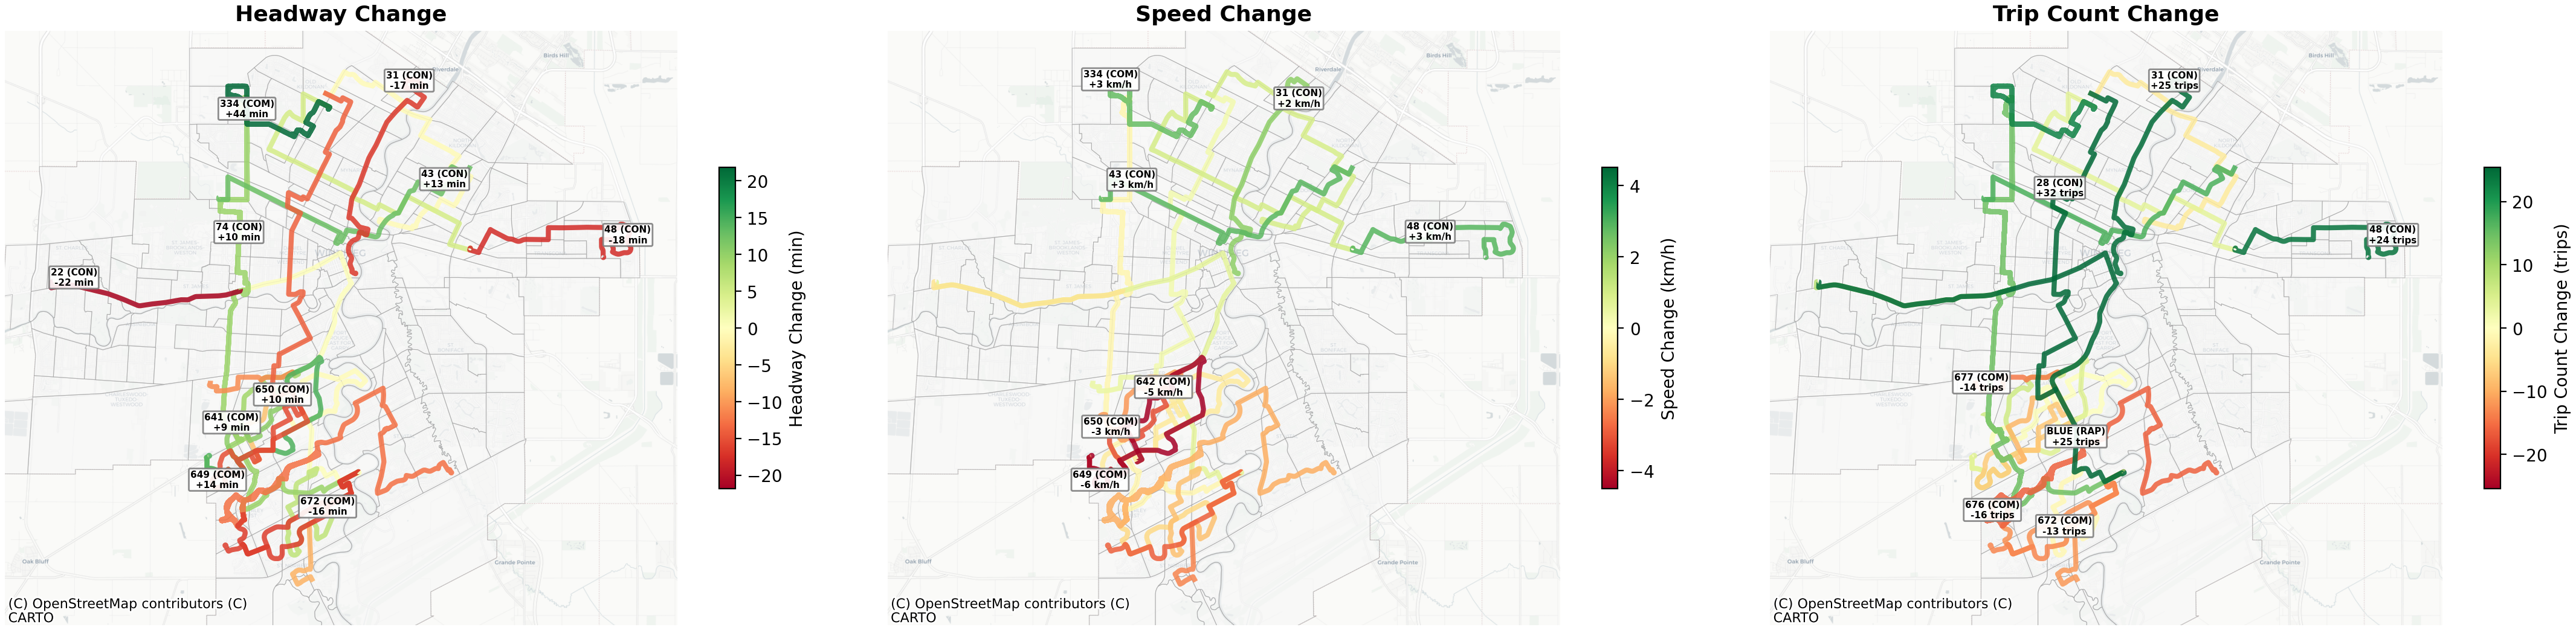
\includegraphics[width=\textwidth]{prepost_combined.png}
    \caption{Route-level impact: headway change (left), speed change (centre), trip count change (right). Green = improved, red = worsened.}
    \label{fig:prepost}
\end{figure}

K-means clustering groups routes into four service archetypes (Figure~\ref{fig:clustering_class}a) and a Random Forest classifier confirms population density as the strongest census predictor of coverage quality (Figure~\ref{fig:clustering_class}b). Pass-up counts identify routes under capacity stress (Figure~\ref{fig:capacity}a); on-time performance maps show peripheral routes are least reliable (Figure~\ref{fig:capacity}b).

\begin{figure}[H]
    \centering
    \begin{subfigure}[b]{0.48\textwidth}
        \centering
        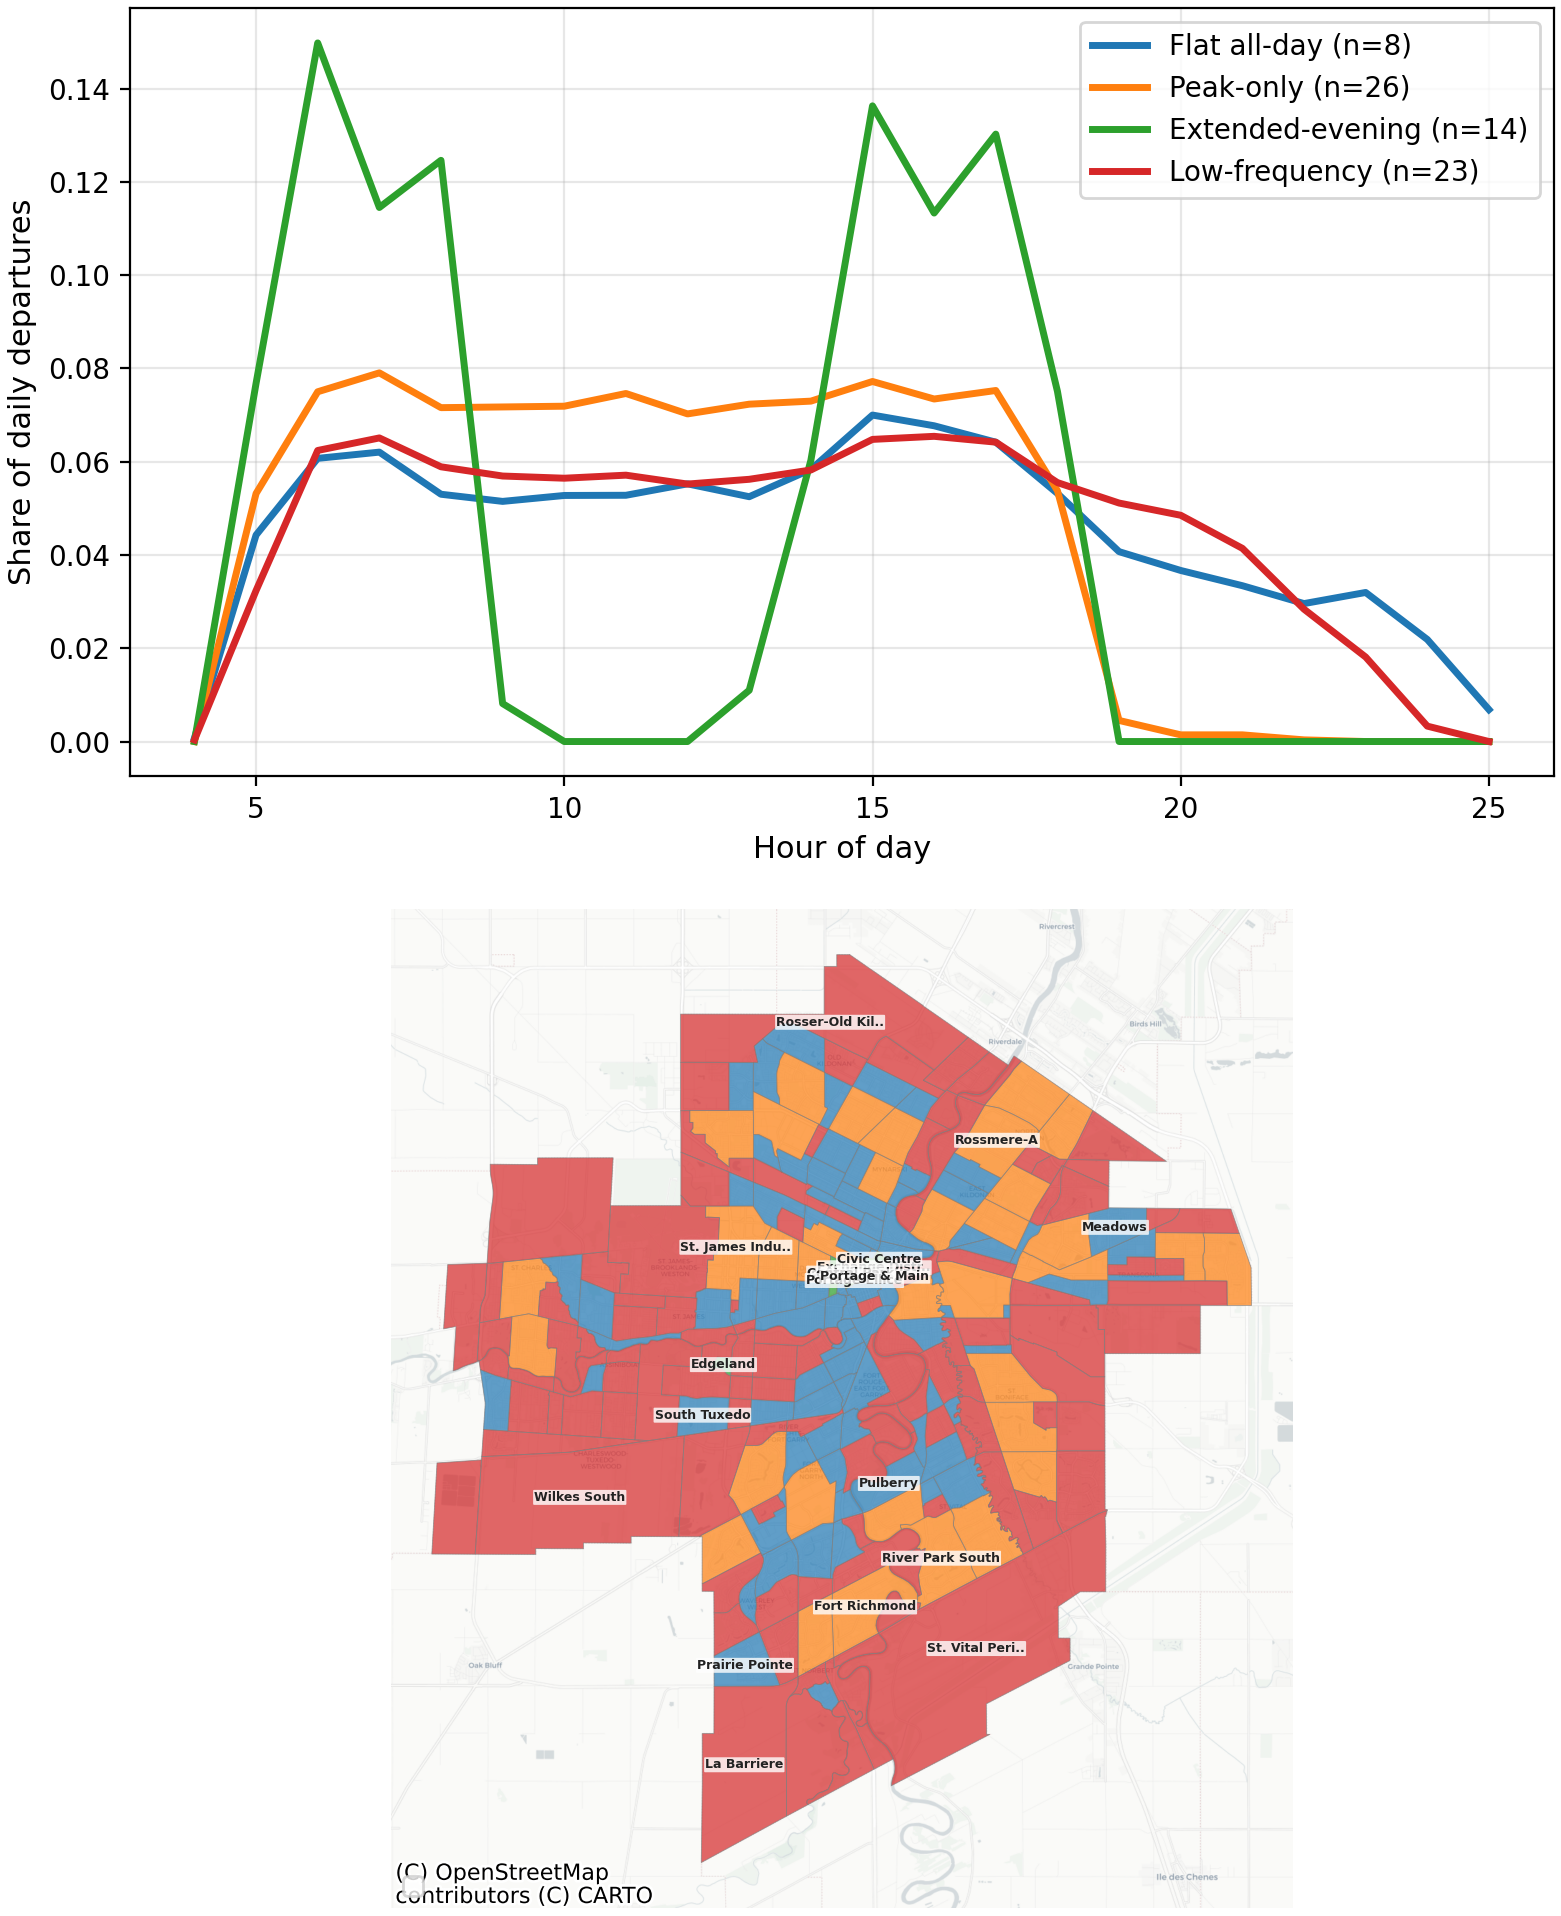
\includegraphics[width=\textwidth]{clustering_combined.png}
        \caption{Route archetypes (top) and neighbourhood service clusters (bottom).}
    \end{subfigure}\hfill
    \begin{subfigure}[b]{0.48\textwidth}
        \centering
        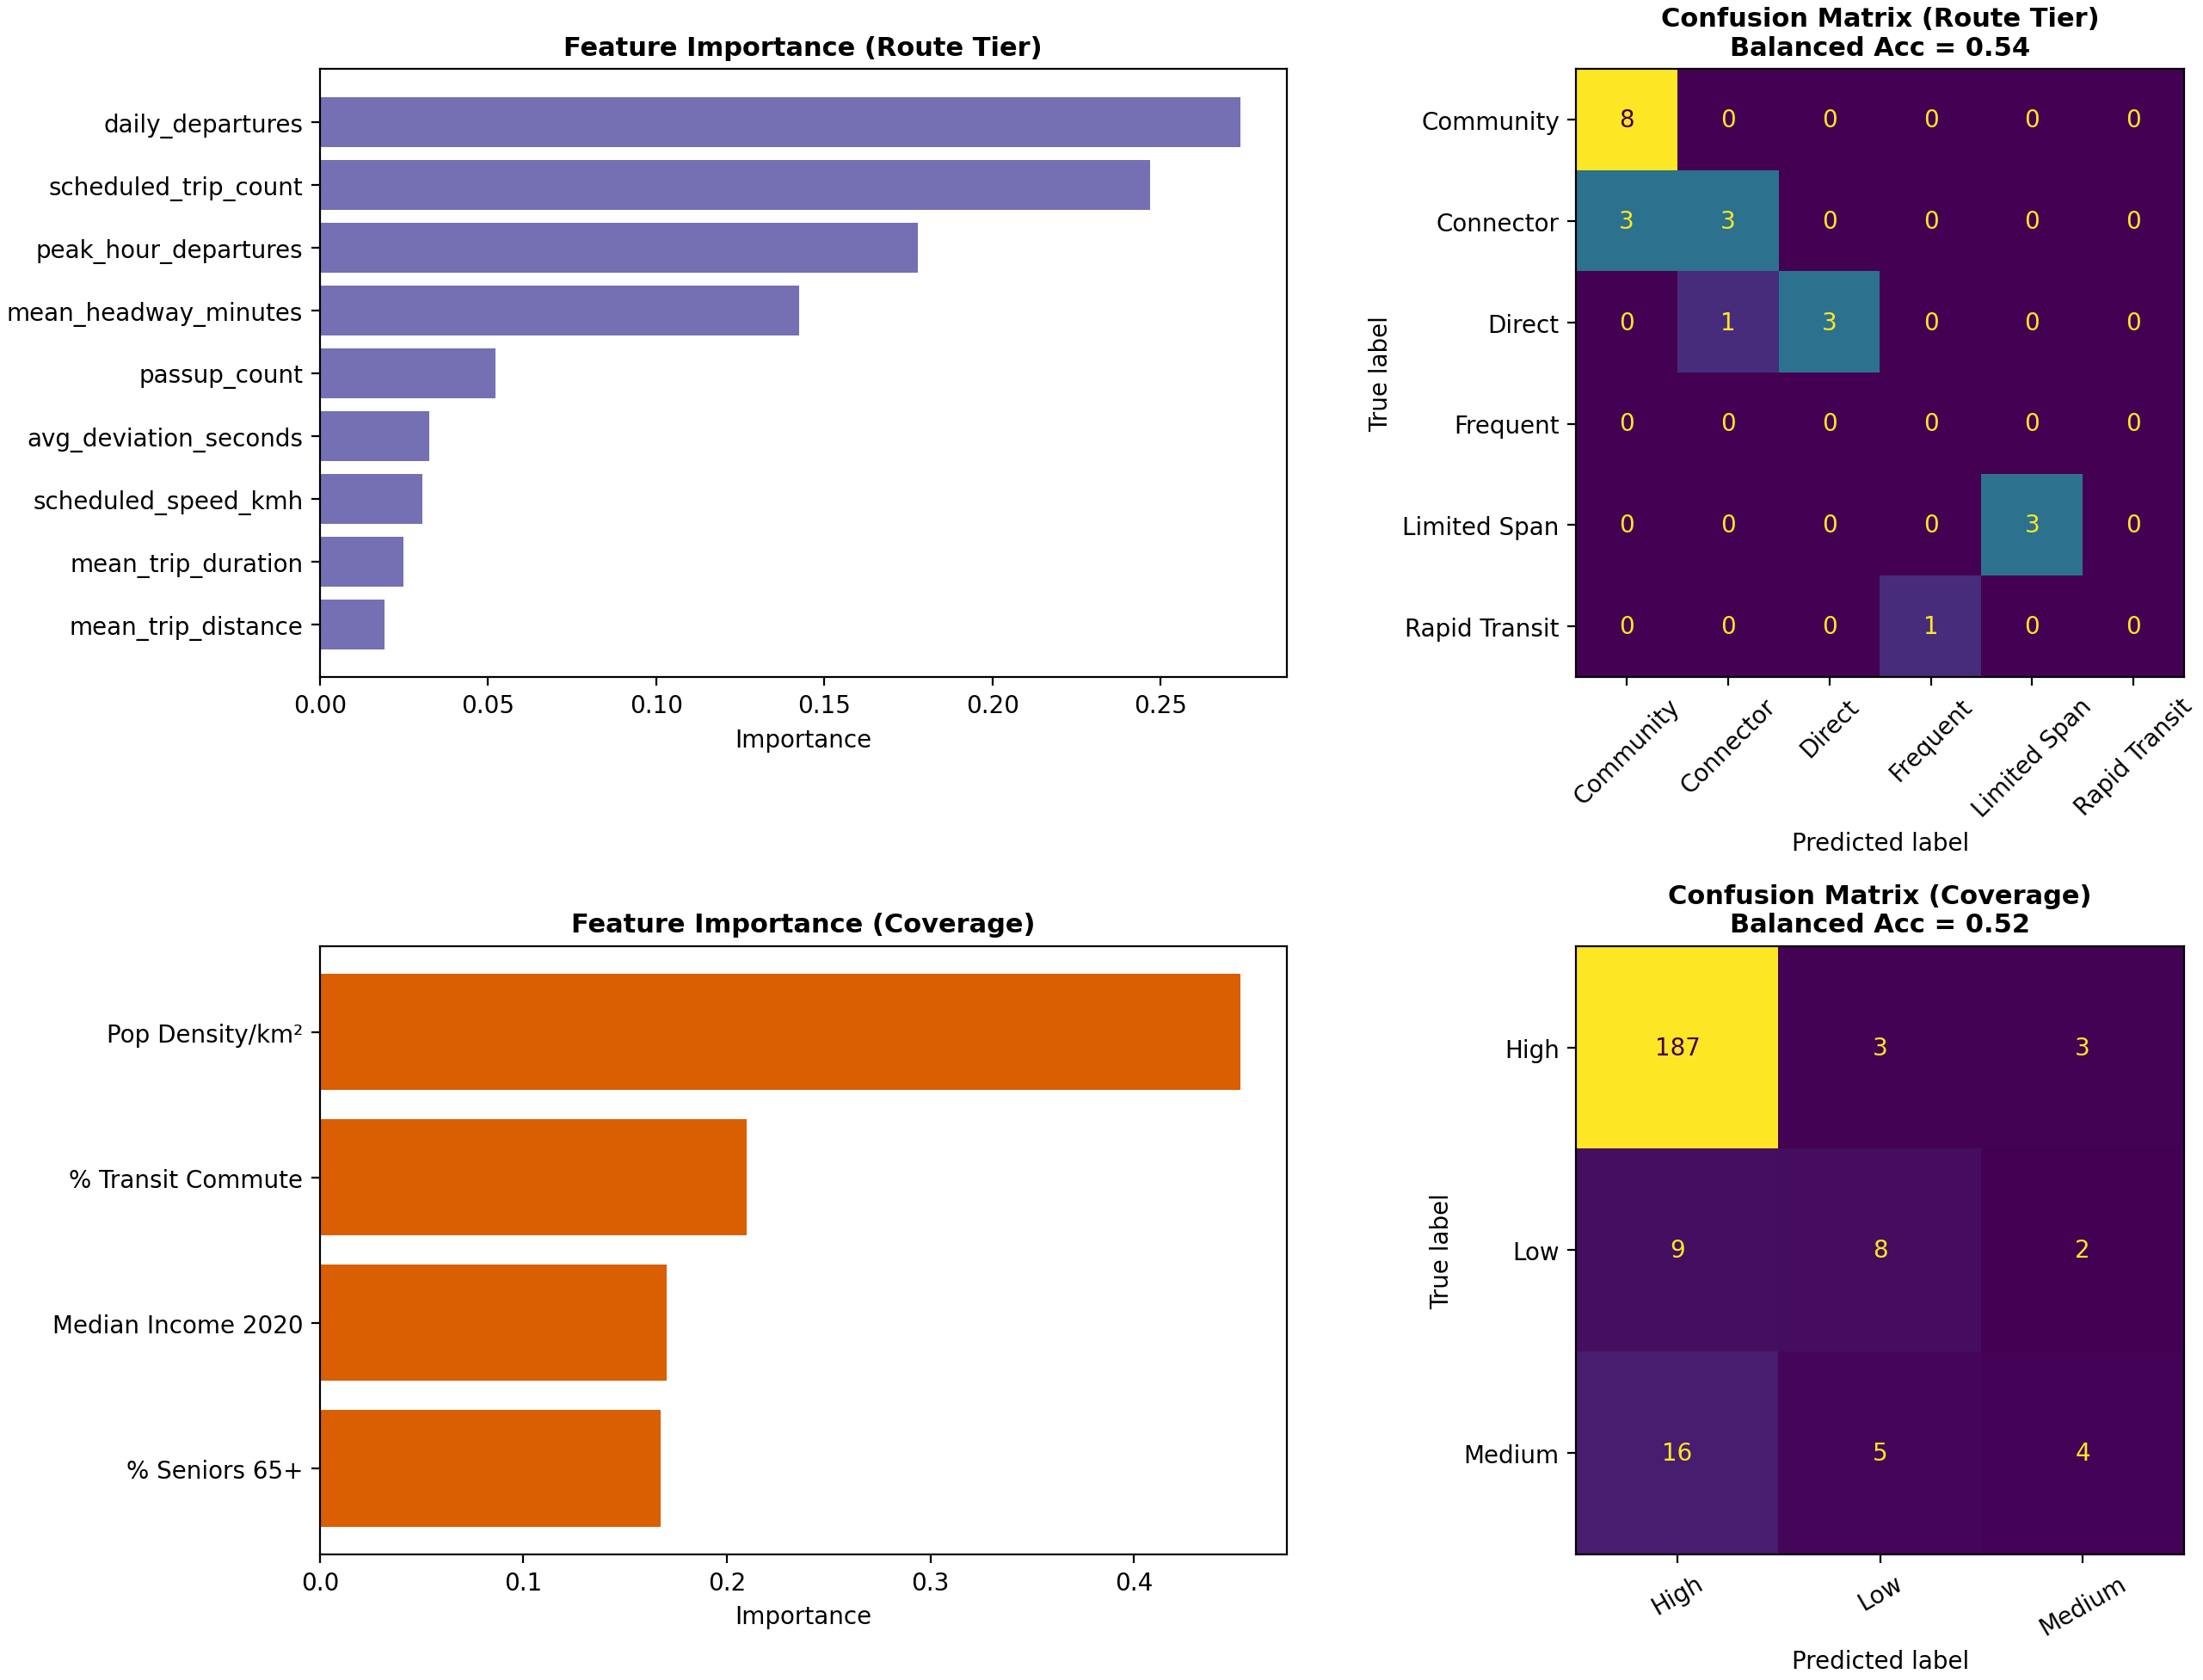
\includegraphics[width=\textwidth]{classification_combined.png}
        \caption{Feature importance and confusion matrices for tier and coverage classifiers.}
    \end{subfigure}
    \caption{Clustering and classification results.}
    \label{fig:clustering_class}
\end{figure}

\begin{figure}[H]
    \centering
    \begin{subfigure}[t]{0.48\textwidth}
        \centering
        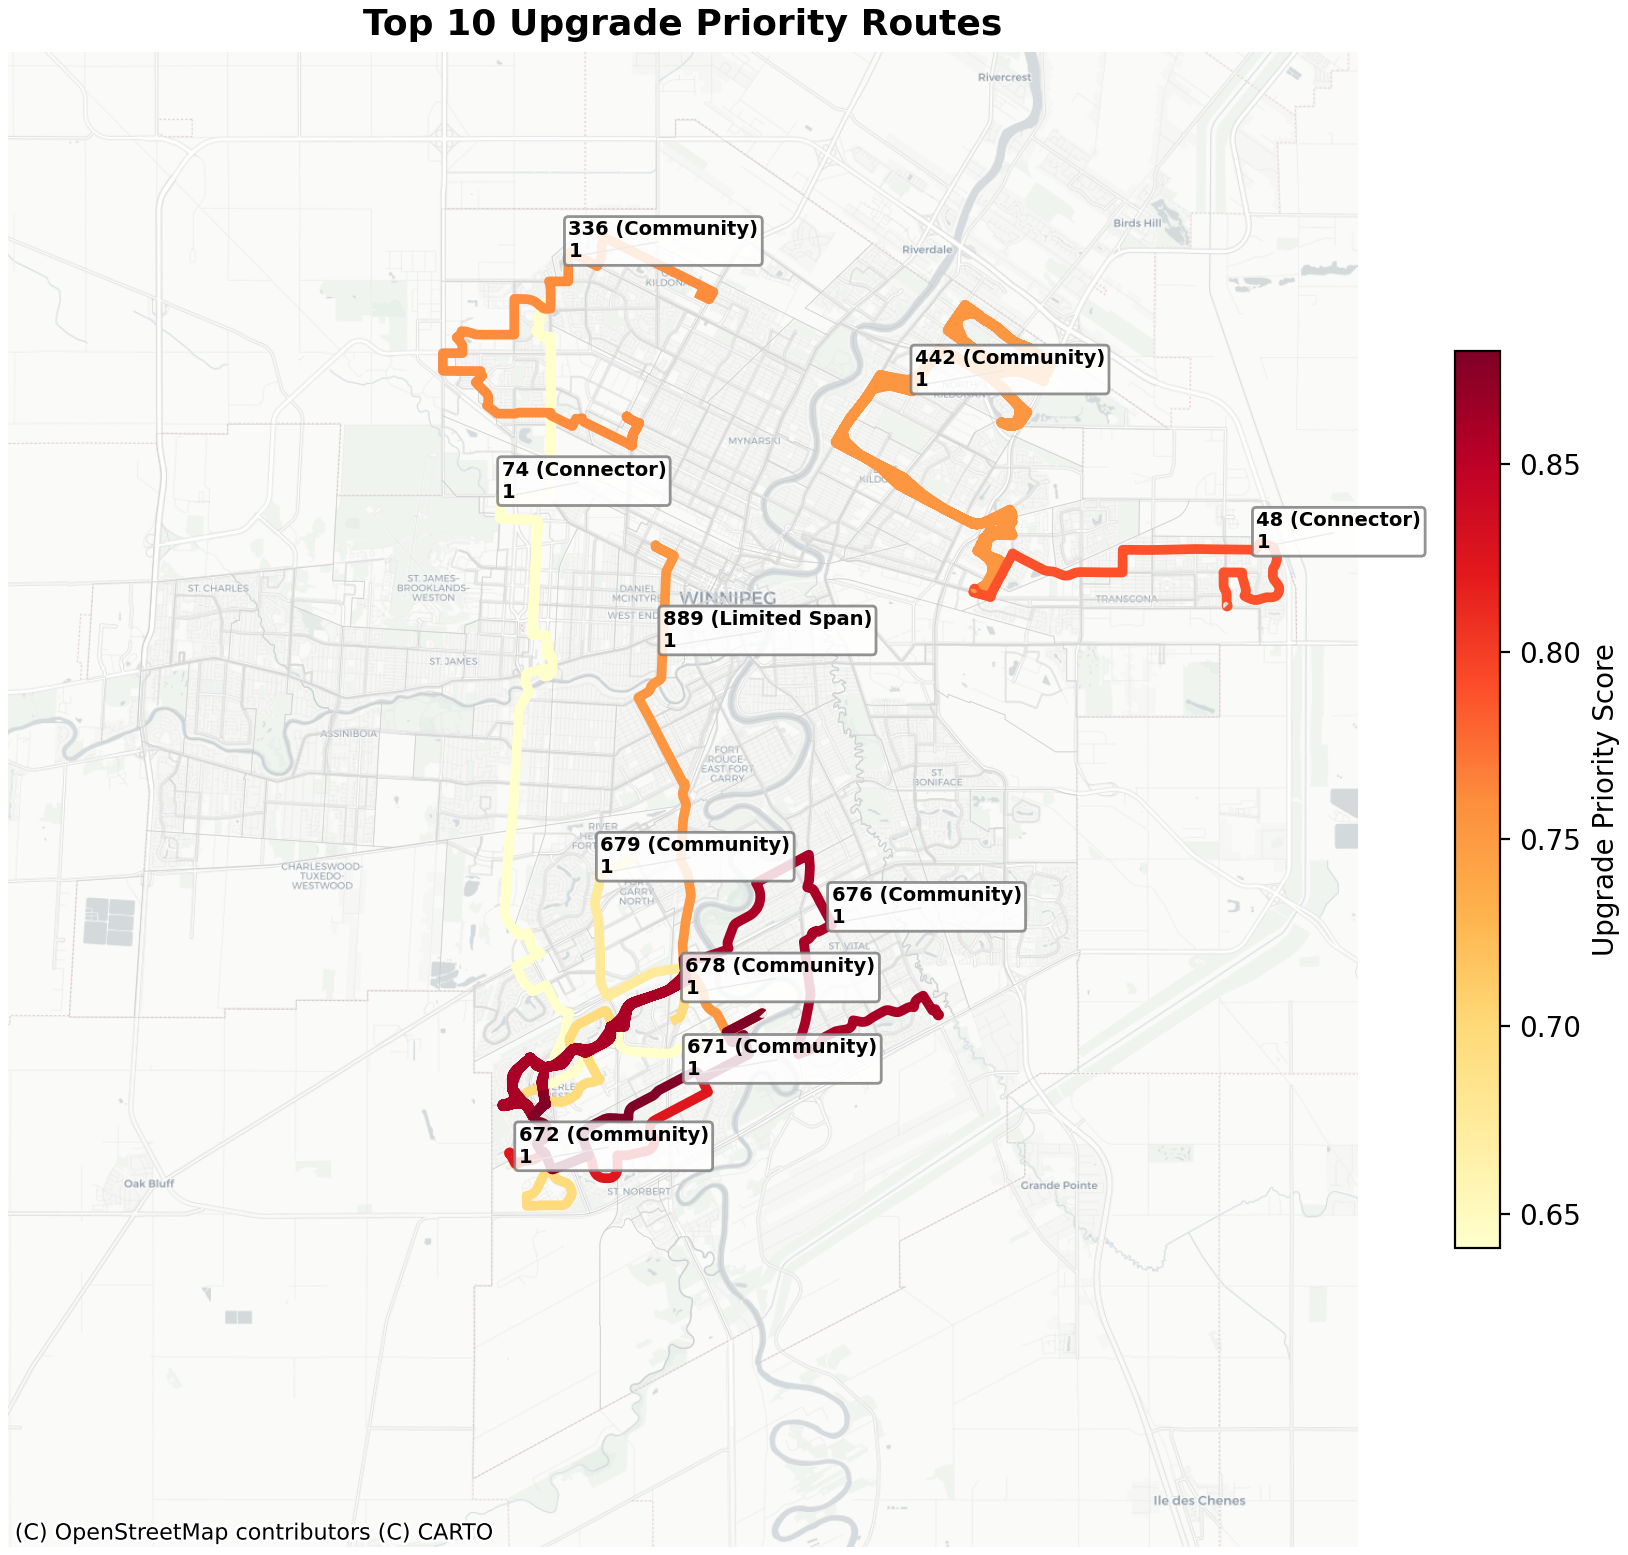
\includegraphics[width=\textwidth,height=6cm,keepaspectratio]{upgrade_priority.png}
        \caption{Top 10 routes by upgrade priority score.}
    \end{subfigure}\hfill
    \begin{subfigure}[t]{0.48\textwidth}
        \centering
        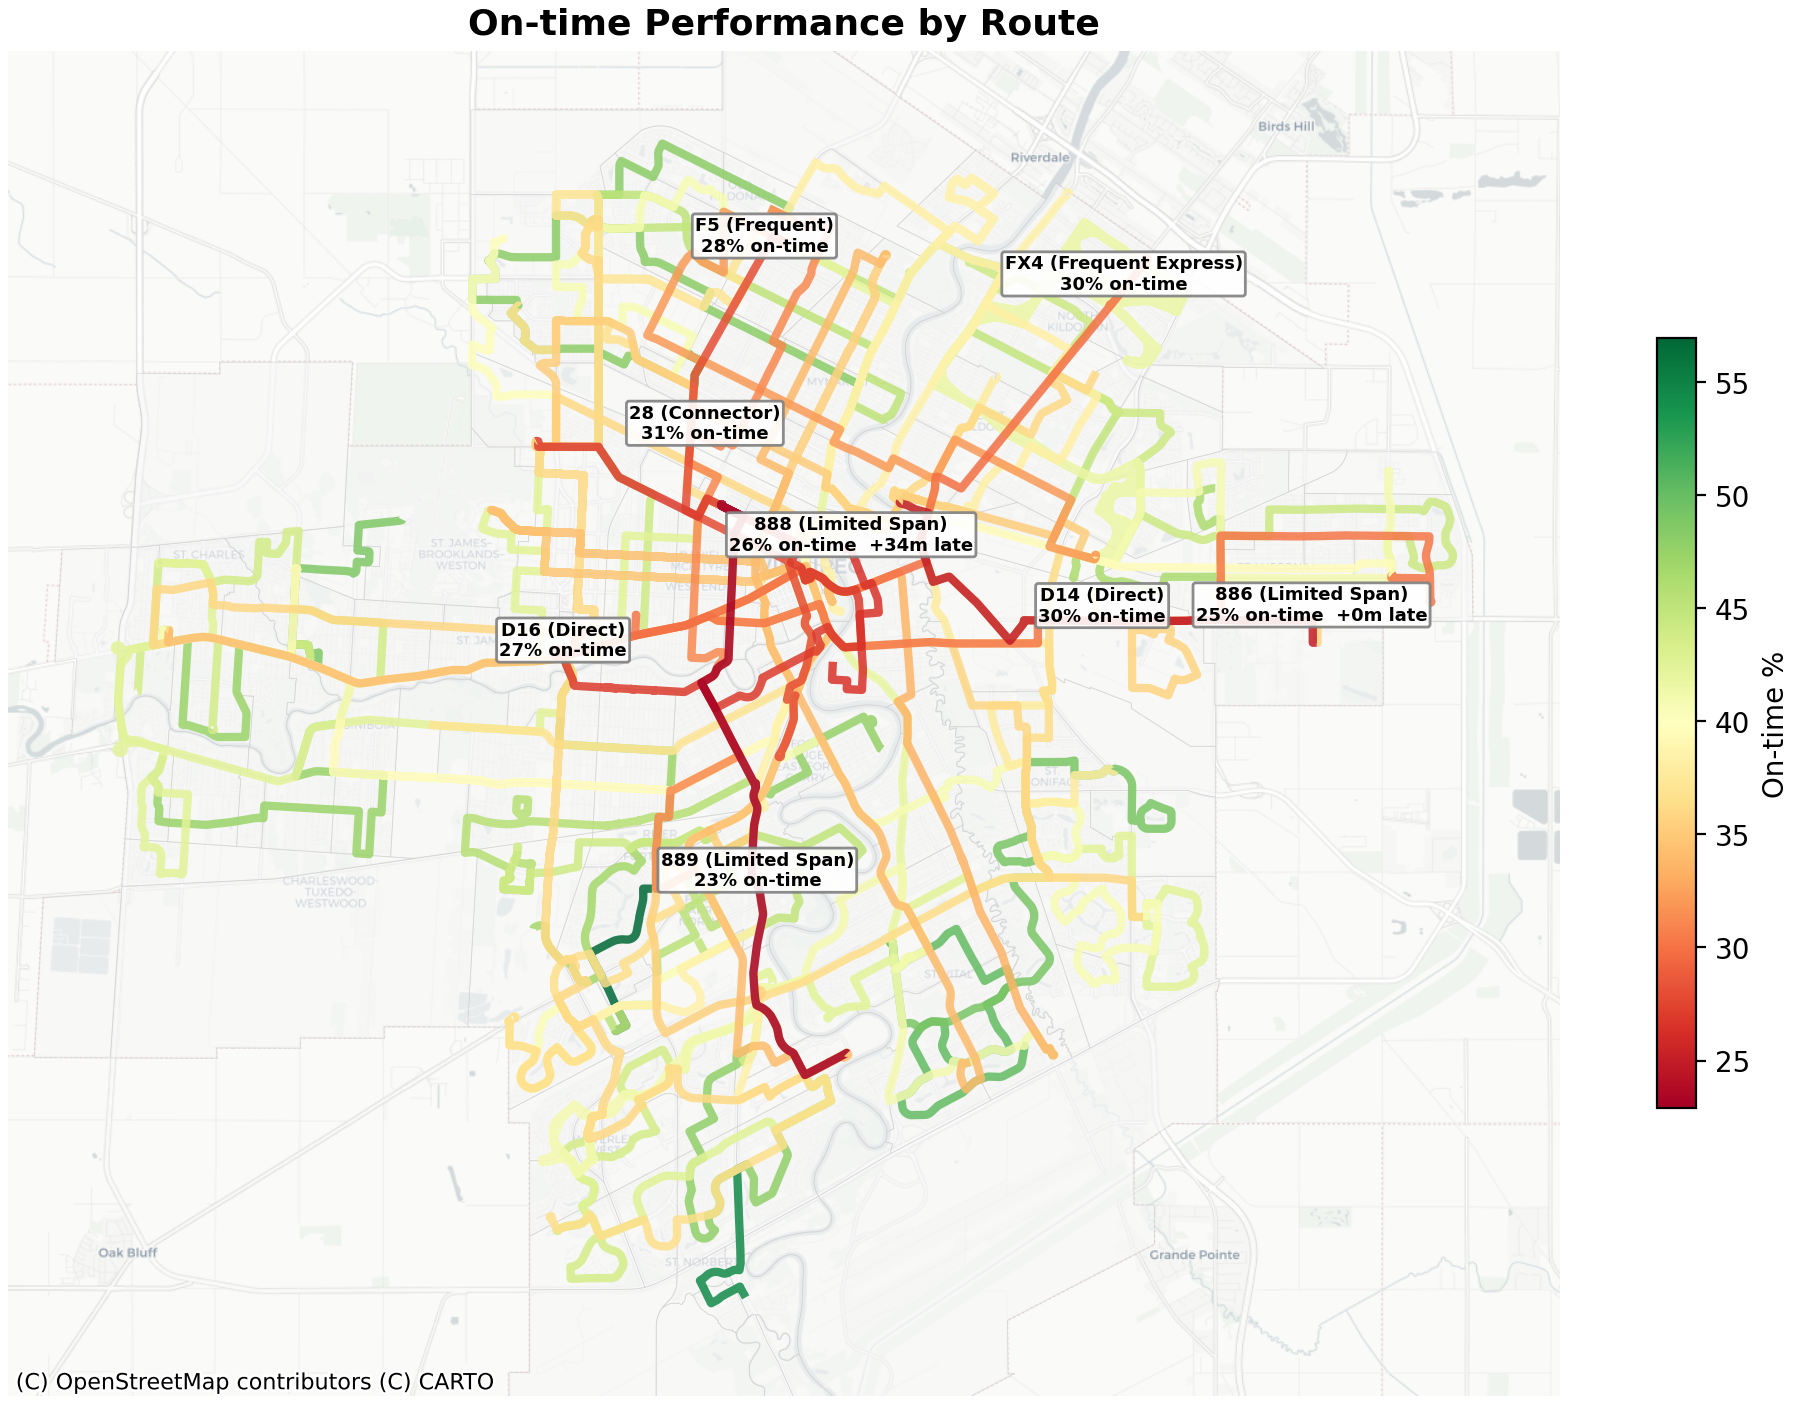
\includegraphics[width=\textwidth,height=6cm,keepaspectratio]{reliability_ontime.png}
        \caption{On-time performance by route.}
    \end{subfigure}
    \caption{Capacity stress and reliability analysis.}
    \label{fig:capacity}
\end{figure}

A 2$\times$3 equity panel (Figure~\ref{fig:equity_access}) combines TOD gap scores, r5py travel-time matrices, transit commute share, immigrant concentration, and employment access change. Census departure demand aligns well with GTFS scheduled supply (Figure~\ref{fig:demand}).

\begin{figure}[H]
    \centering
    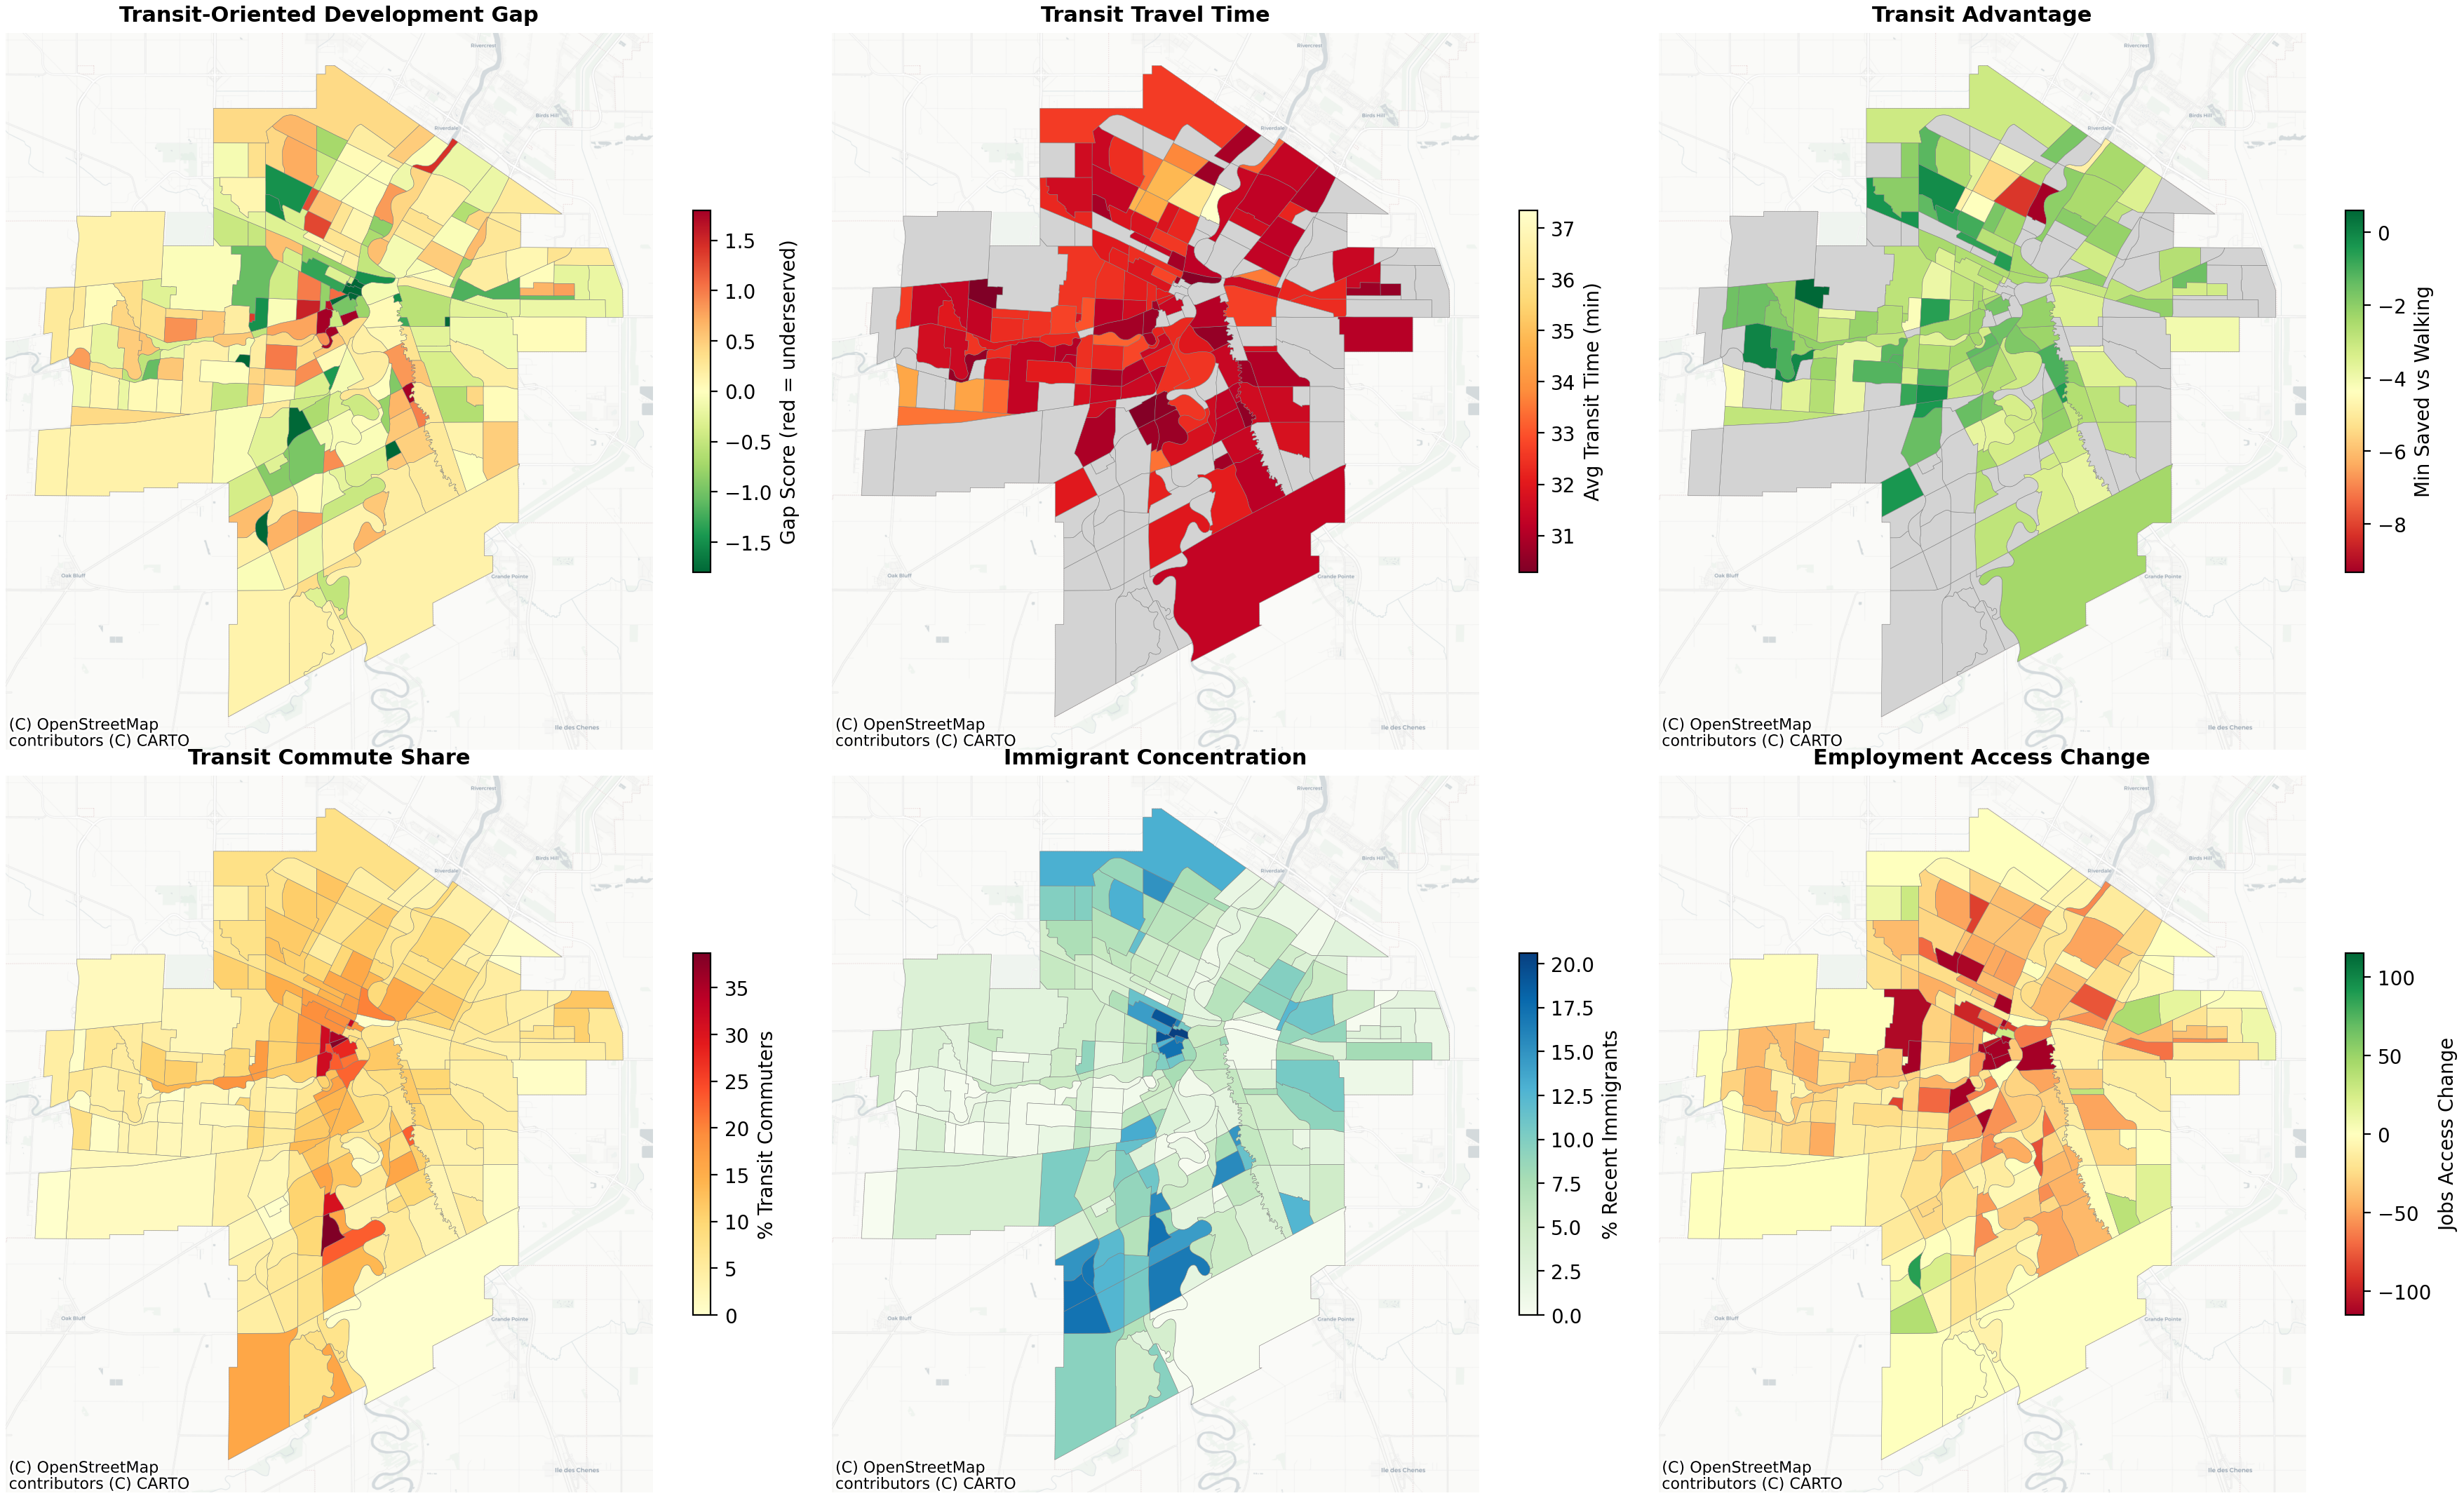
\includegraphics[width=0.85\textwidth]{equity_combined.png}
    \caption{Equity and accessibility (2$\times$3). Top: TOD gap score, transit travel time, transit time savings vs walking. Bottom: transit commute share, immigrant concentration, employment access change.}
    \label{fig:equity_access}
\end{figure}

\begin{figure}[H]
    \centering
    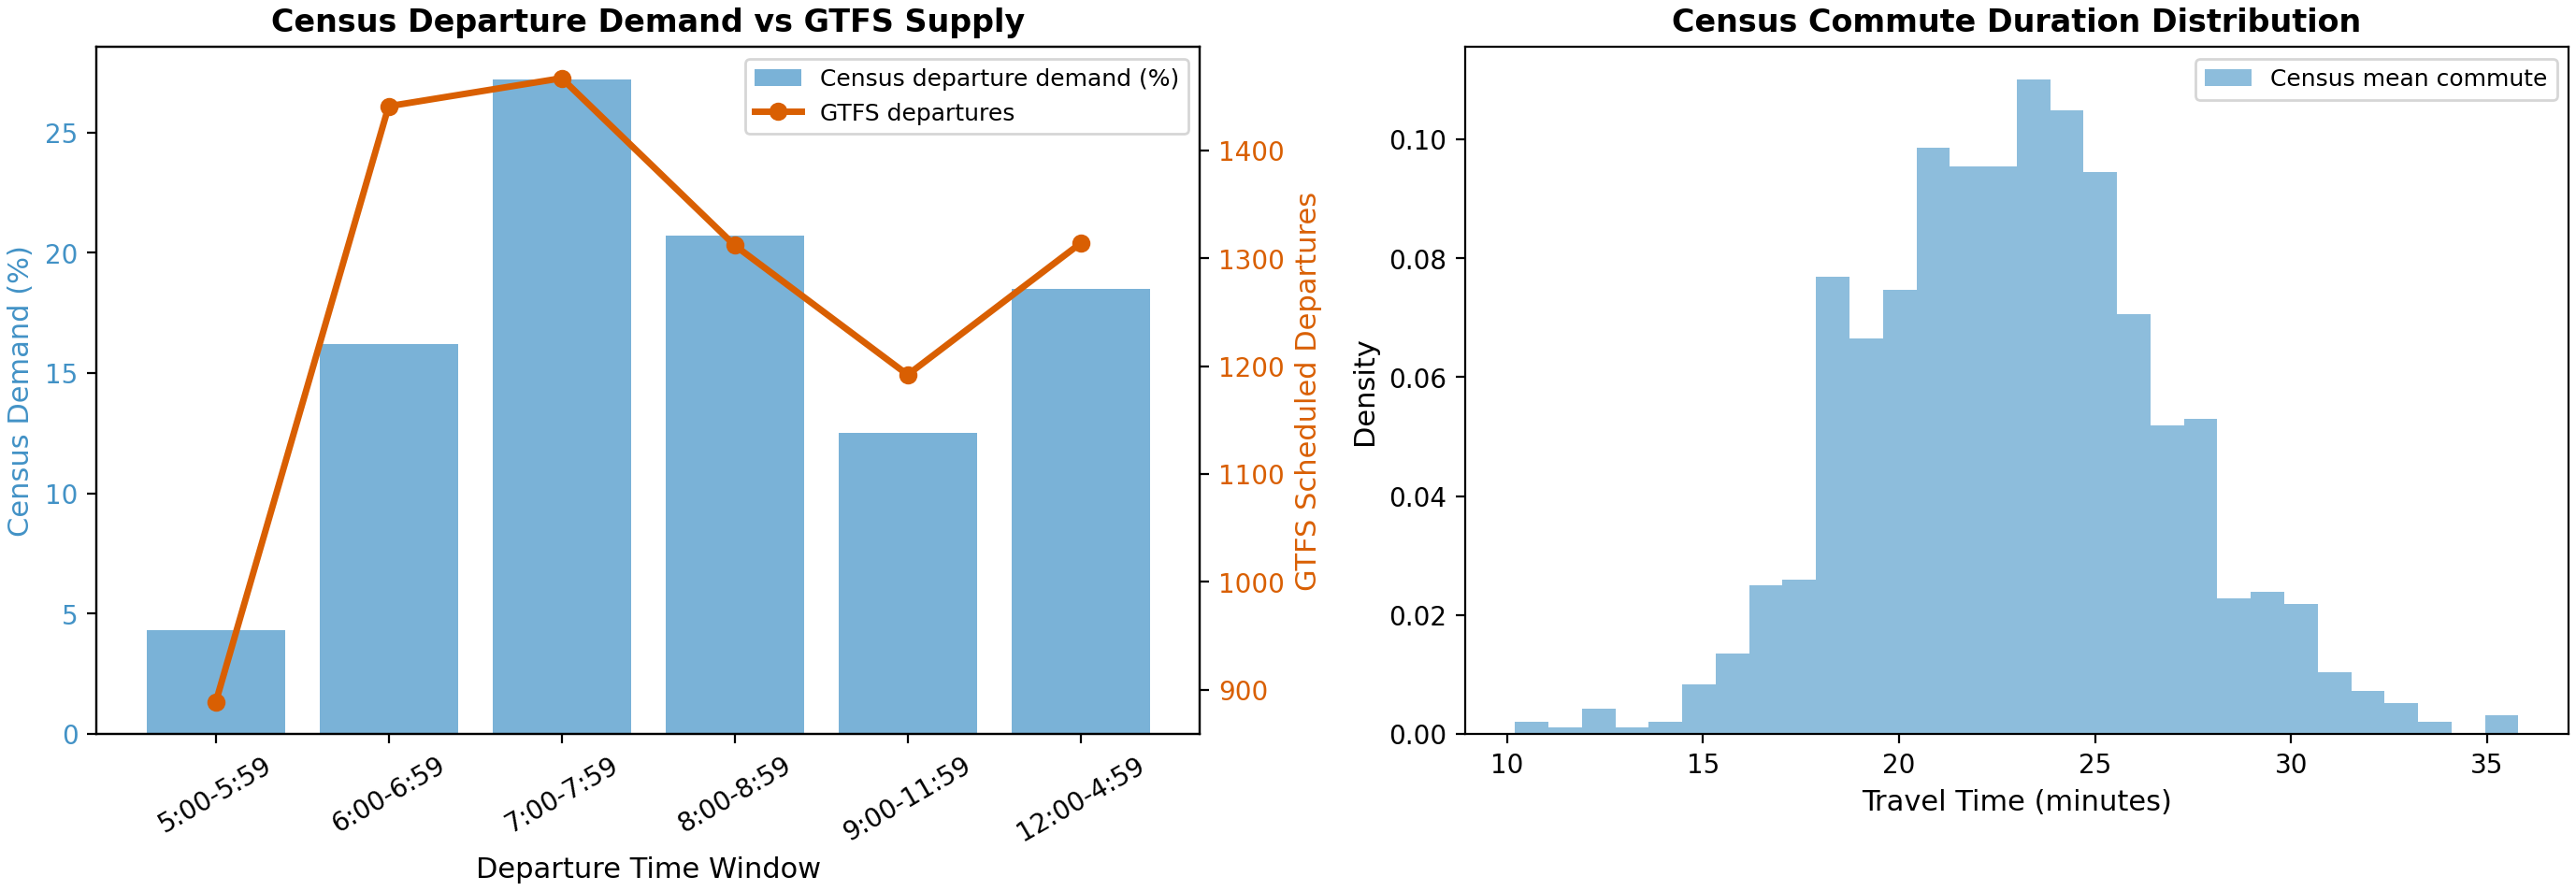
\includegraphics[width=0.72\textwidth]{demand_validation.png}
    \caption{Census departure demand vs GTFS scheduled supply (left) and commute duration distribution (right).}
    \label{fig:demand}
\end{figure}

% ----------------------------------------
\subsection{Network Analysis (Cathy)}

Cathy modelled the transit network as a directed graph using NetworkX and city2graph. Network metrics were compared before and after the PTN overhaul (Figure~\ref{fig:network}a), showing 25\% fewer nodes but 18\% higher density. A transfer burden heatmap (Figure~\ref{fig:network}b) reveals which hub pairs require the most transfers. Hub ranking by degree centrality identifies the backbone stops, while Louvain community detection clusters stops into 15 service regions that align with neighbourhood boundaries (Figure~\ref{fig:communities}).

\begin{figure}[H]
    \centering
    \begin{subfigure}[t]{0.48\textwidth}
        \centering
        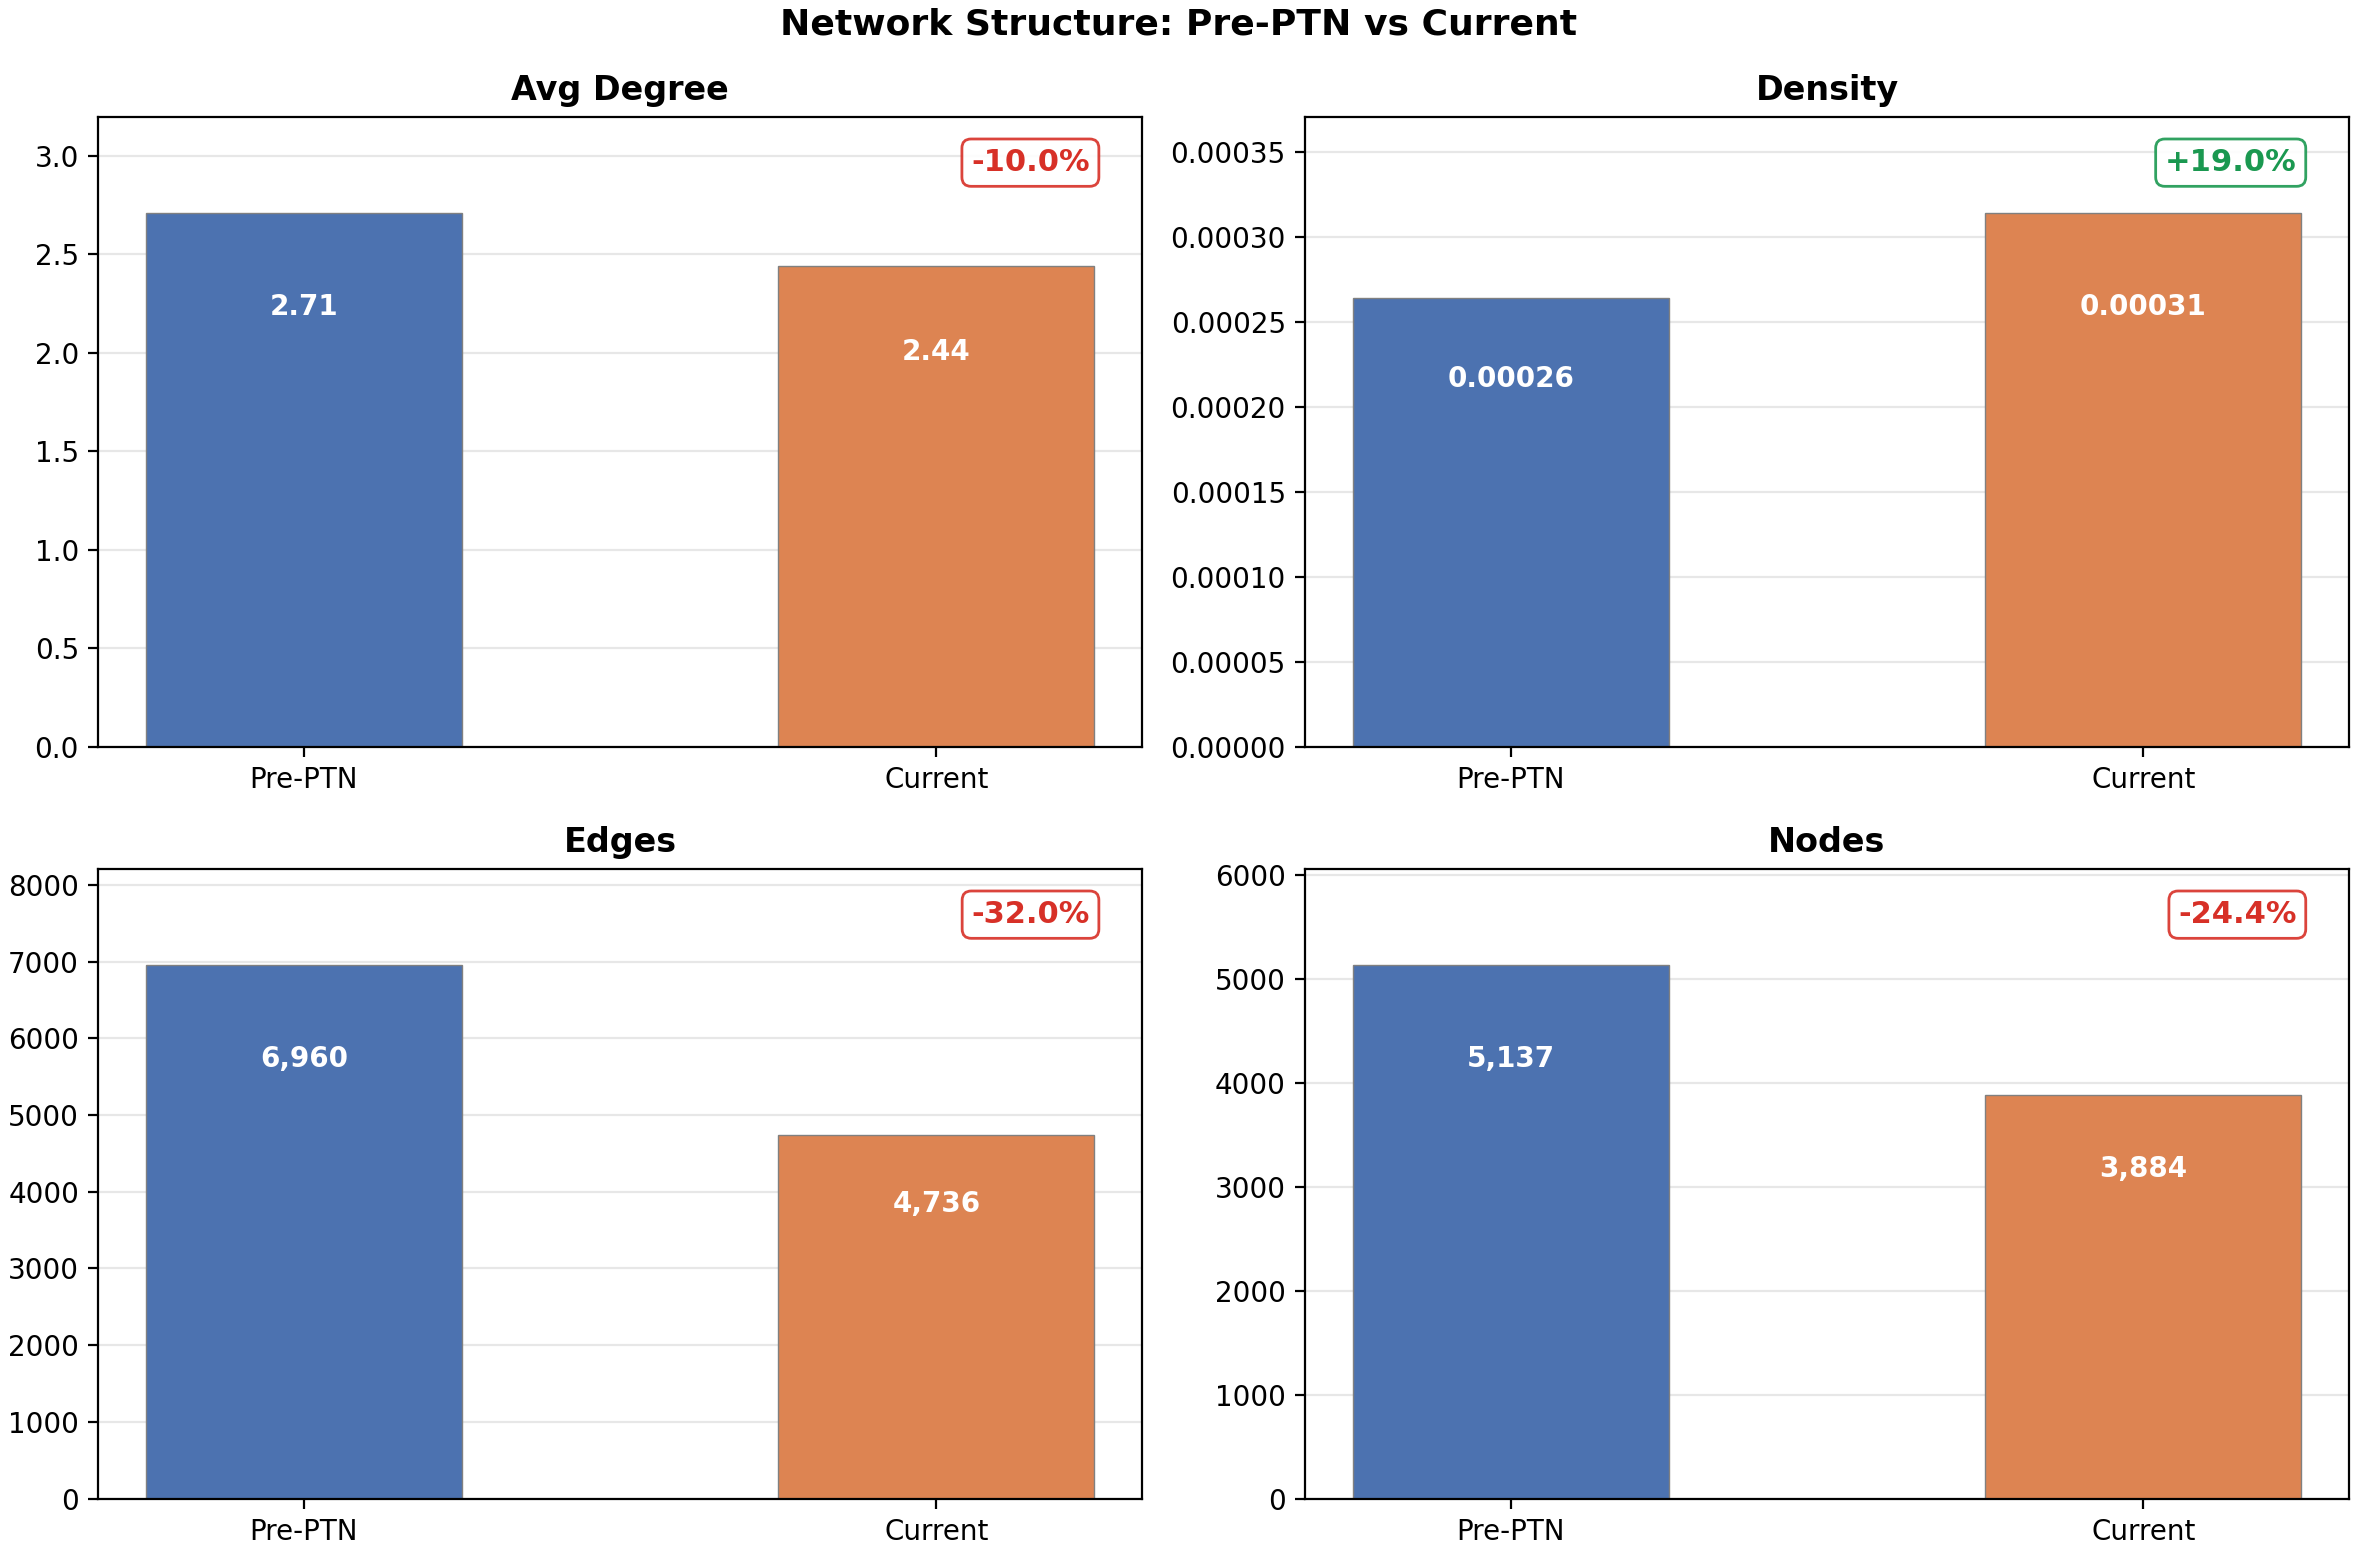
\includegraphics[height=5cm]{network_metrics_prepost.png}
        \caption{Network metrics before and after PTN.}
    \end{subfigure}\hfill
    \begin{subfigure}[t]{0.48\textwidth}
        \centering
        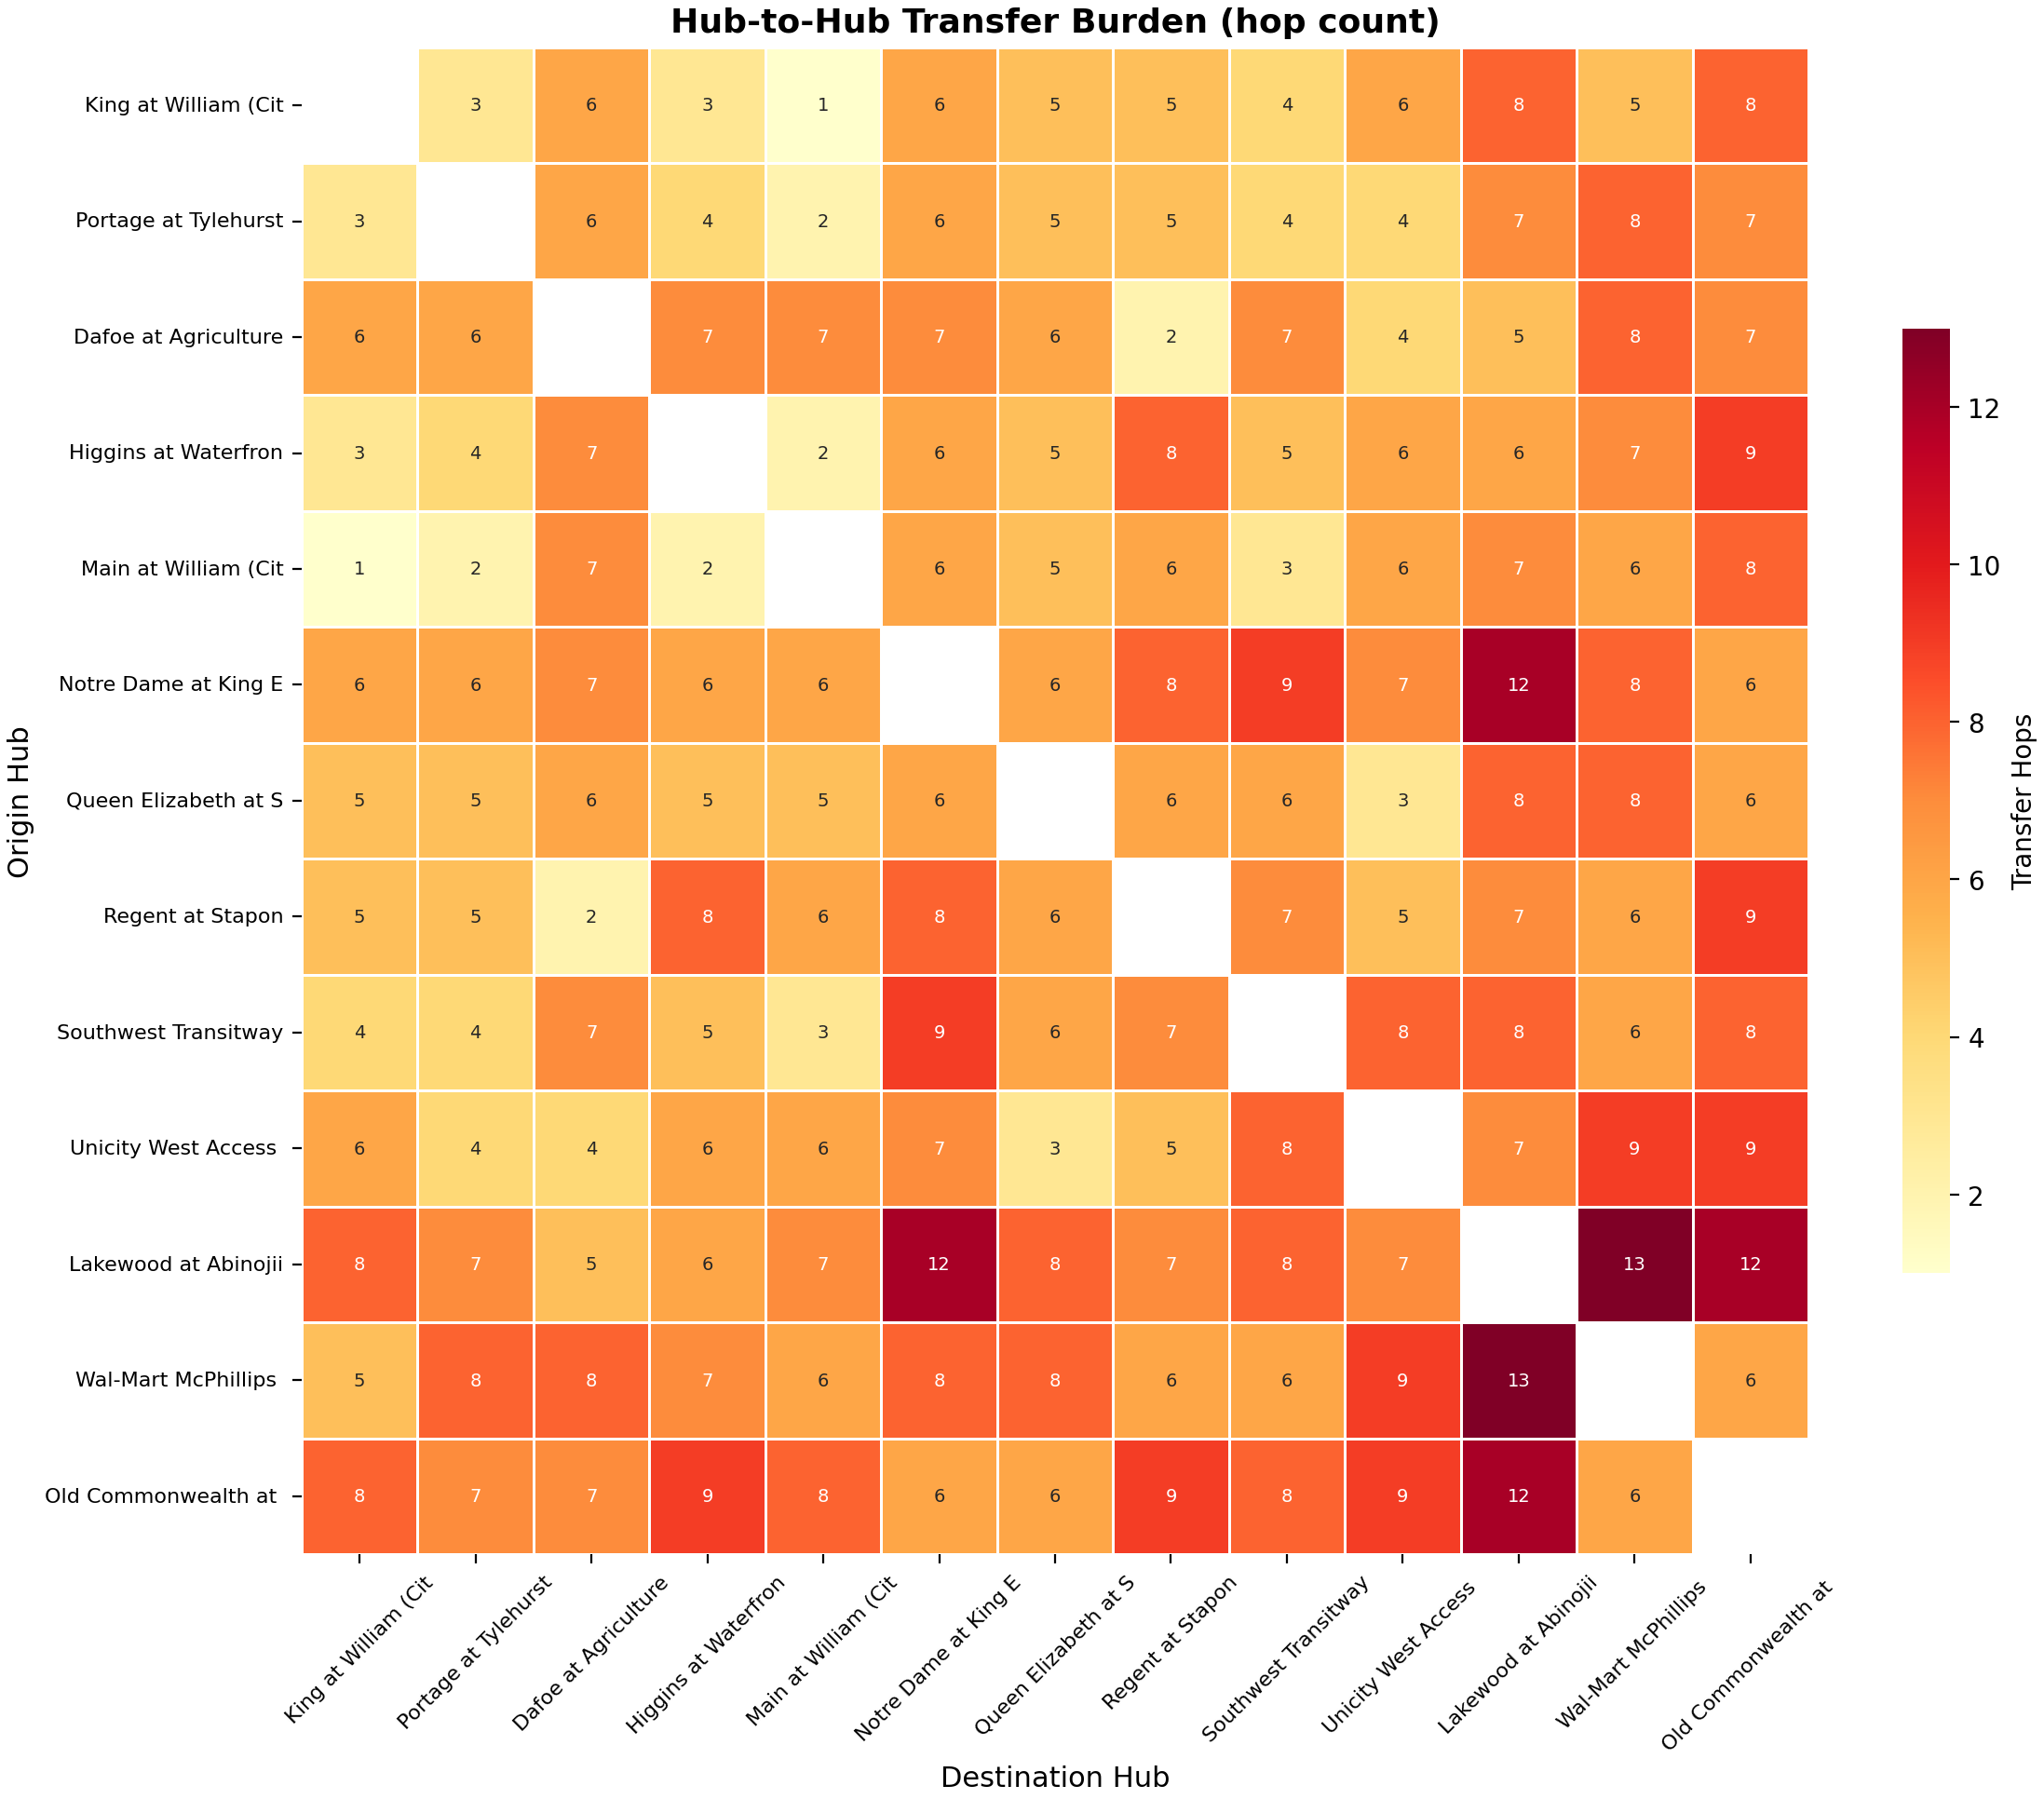
\includegraphics[height=5cm]{transfer_heatmap.png}
        \caption{Hub-to-hub transfer burden (hop count).}
    \end{subfigure}
    \caption{Network structure analysis.}
    \label{fig:network}
\end{figure}

\begin{figure}[H]
    \centering
    \begin{subfigure}[t]{0.48\textwidth}
        \centering
        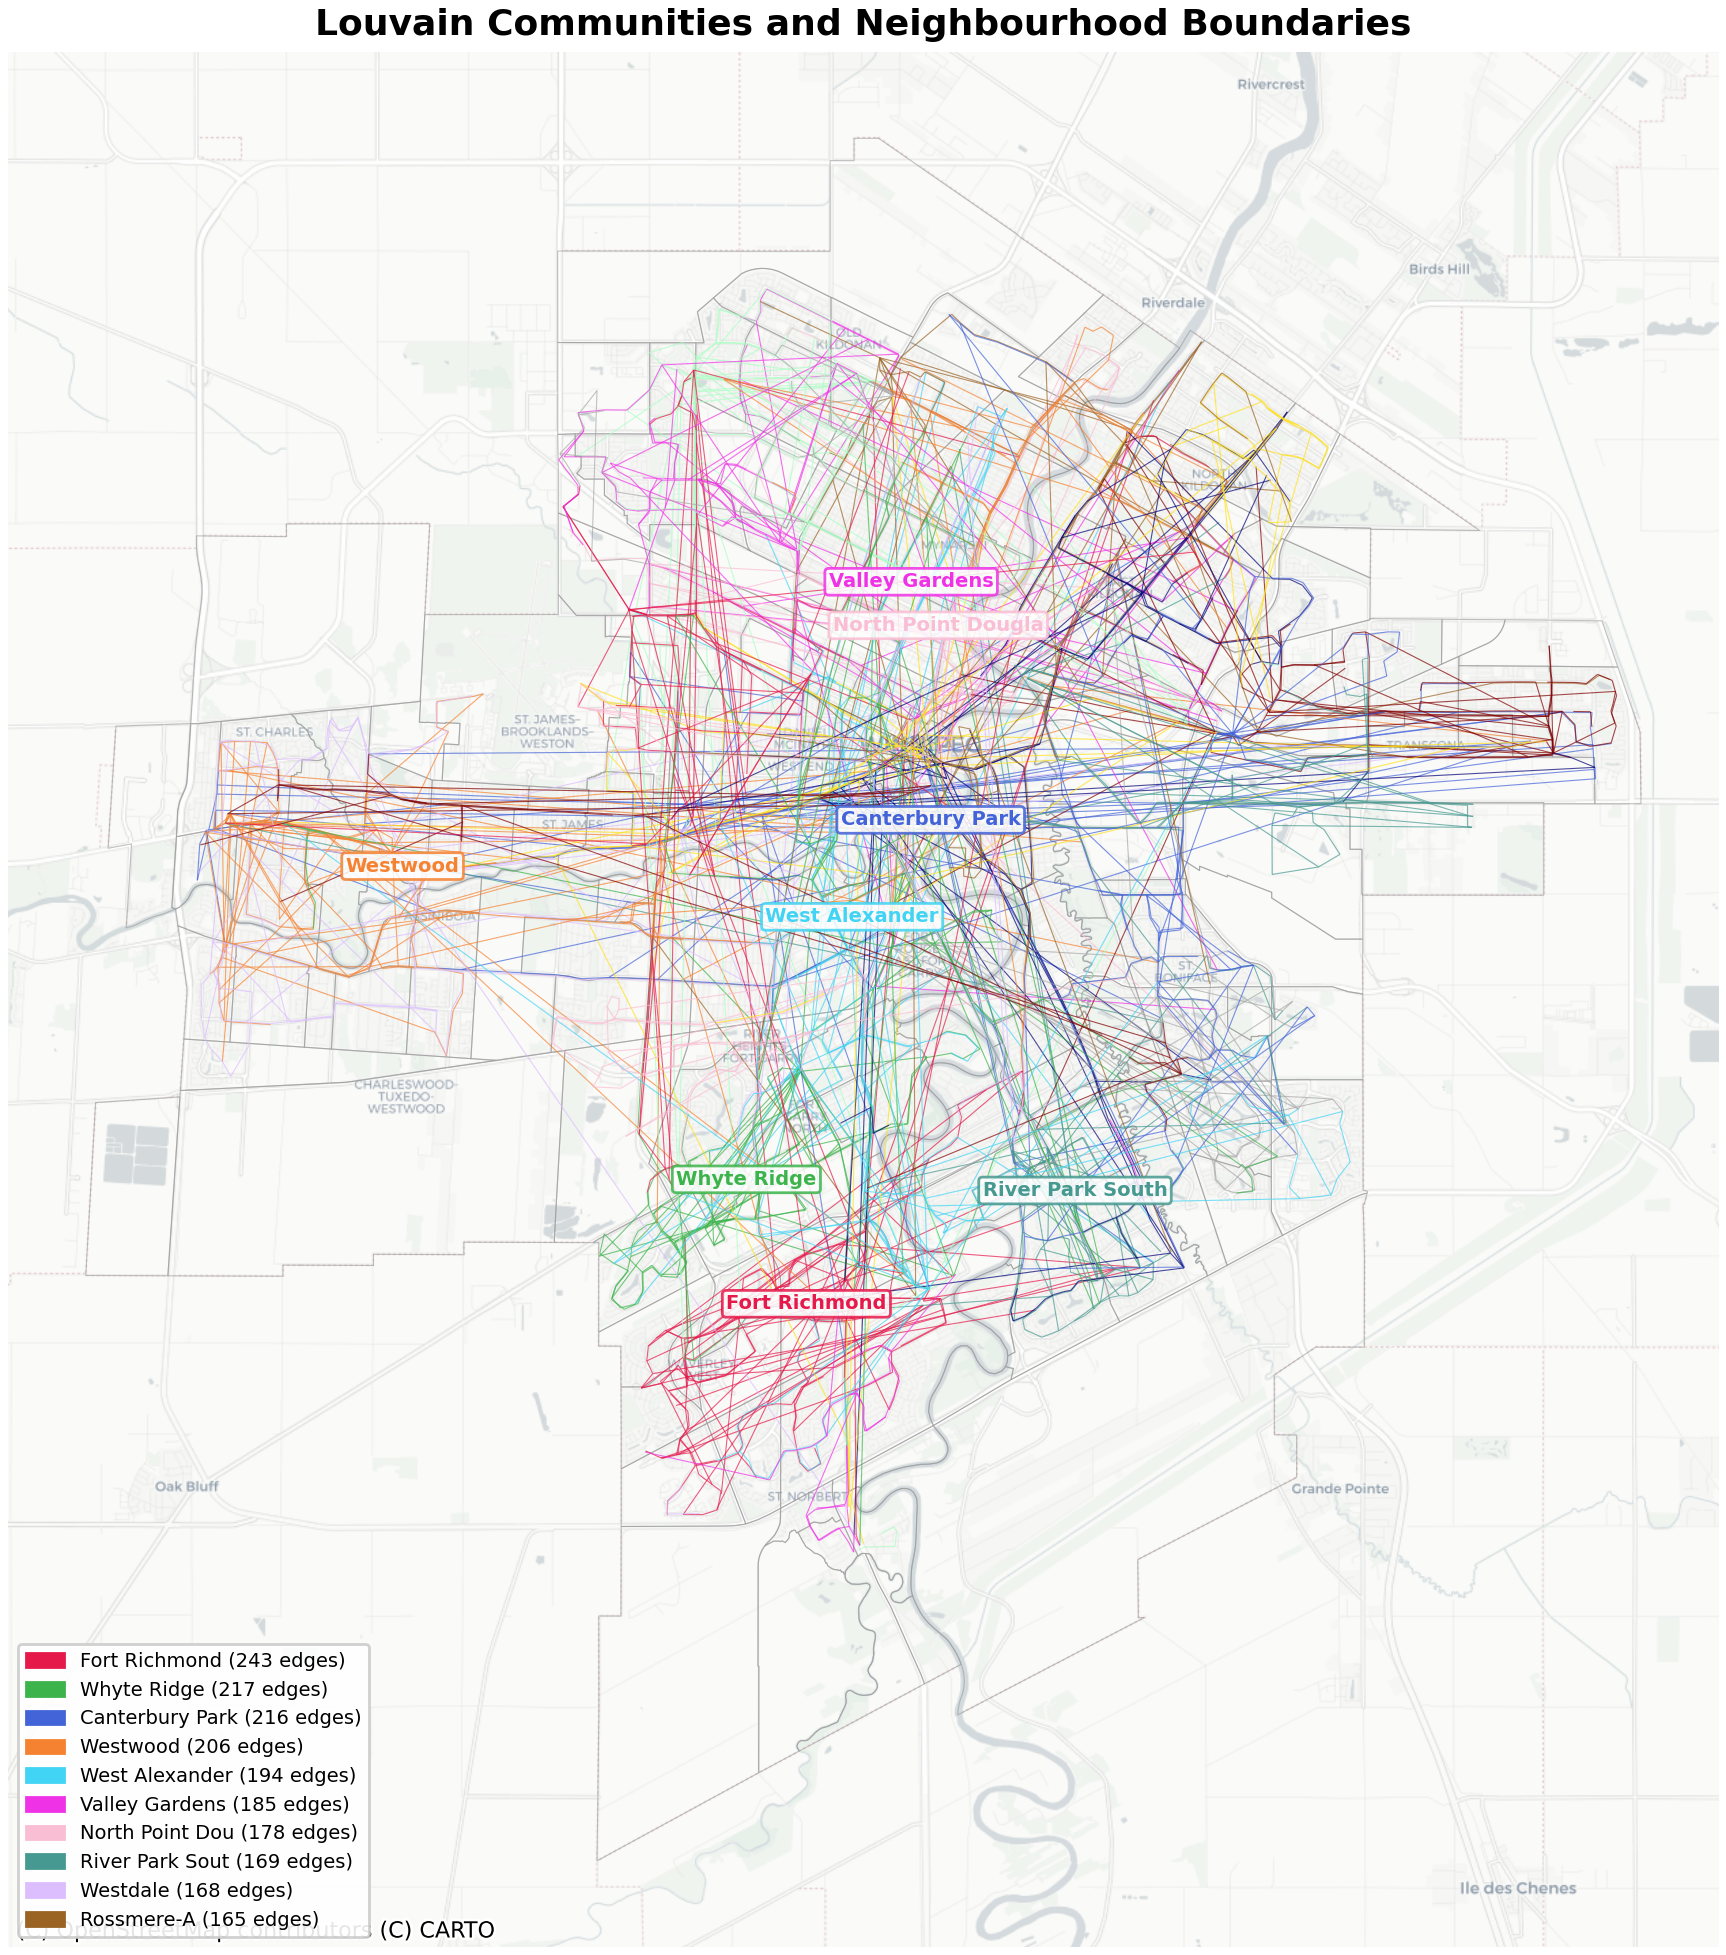
\includegraphics[width=\textwidth,height=7.5cm,keepaspectratio]{community_boundary_alignment.png}
        \caption{Louvain communities with neighbourhood boundaries.}
        \label{fig:communities}
    \end{subfigure}\hfill
    \begin{subfigure}[t]{0.48\textwidth}
        \centering
        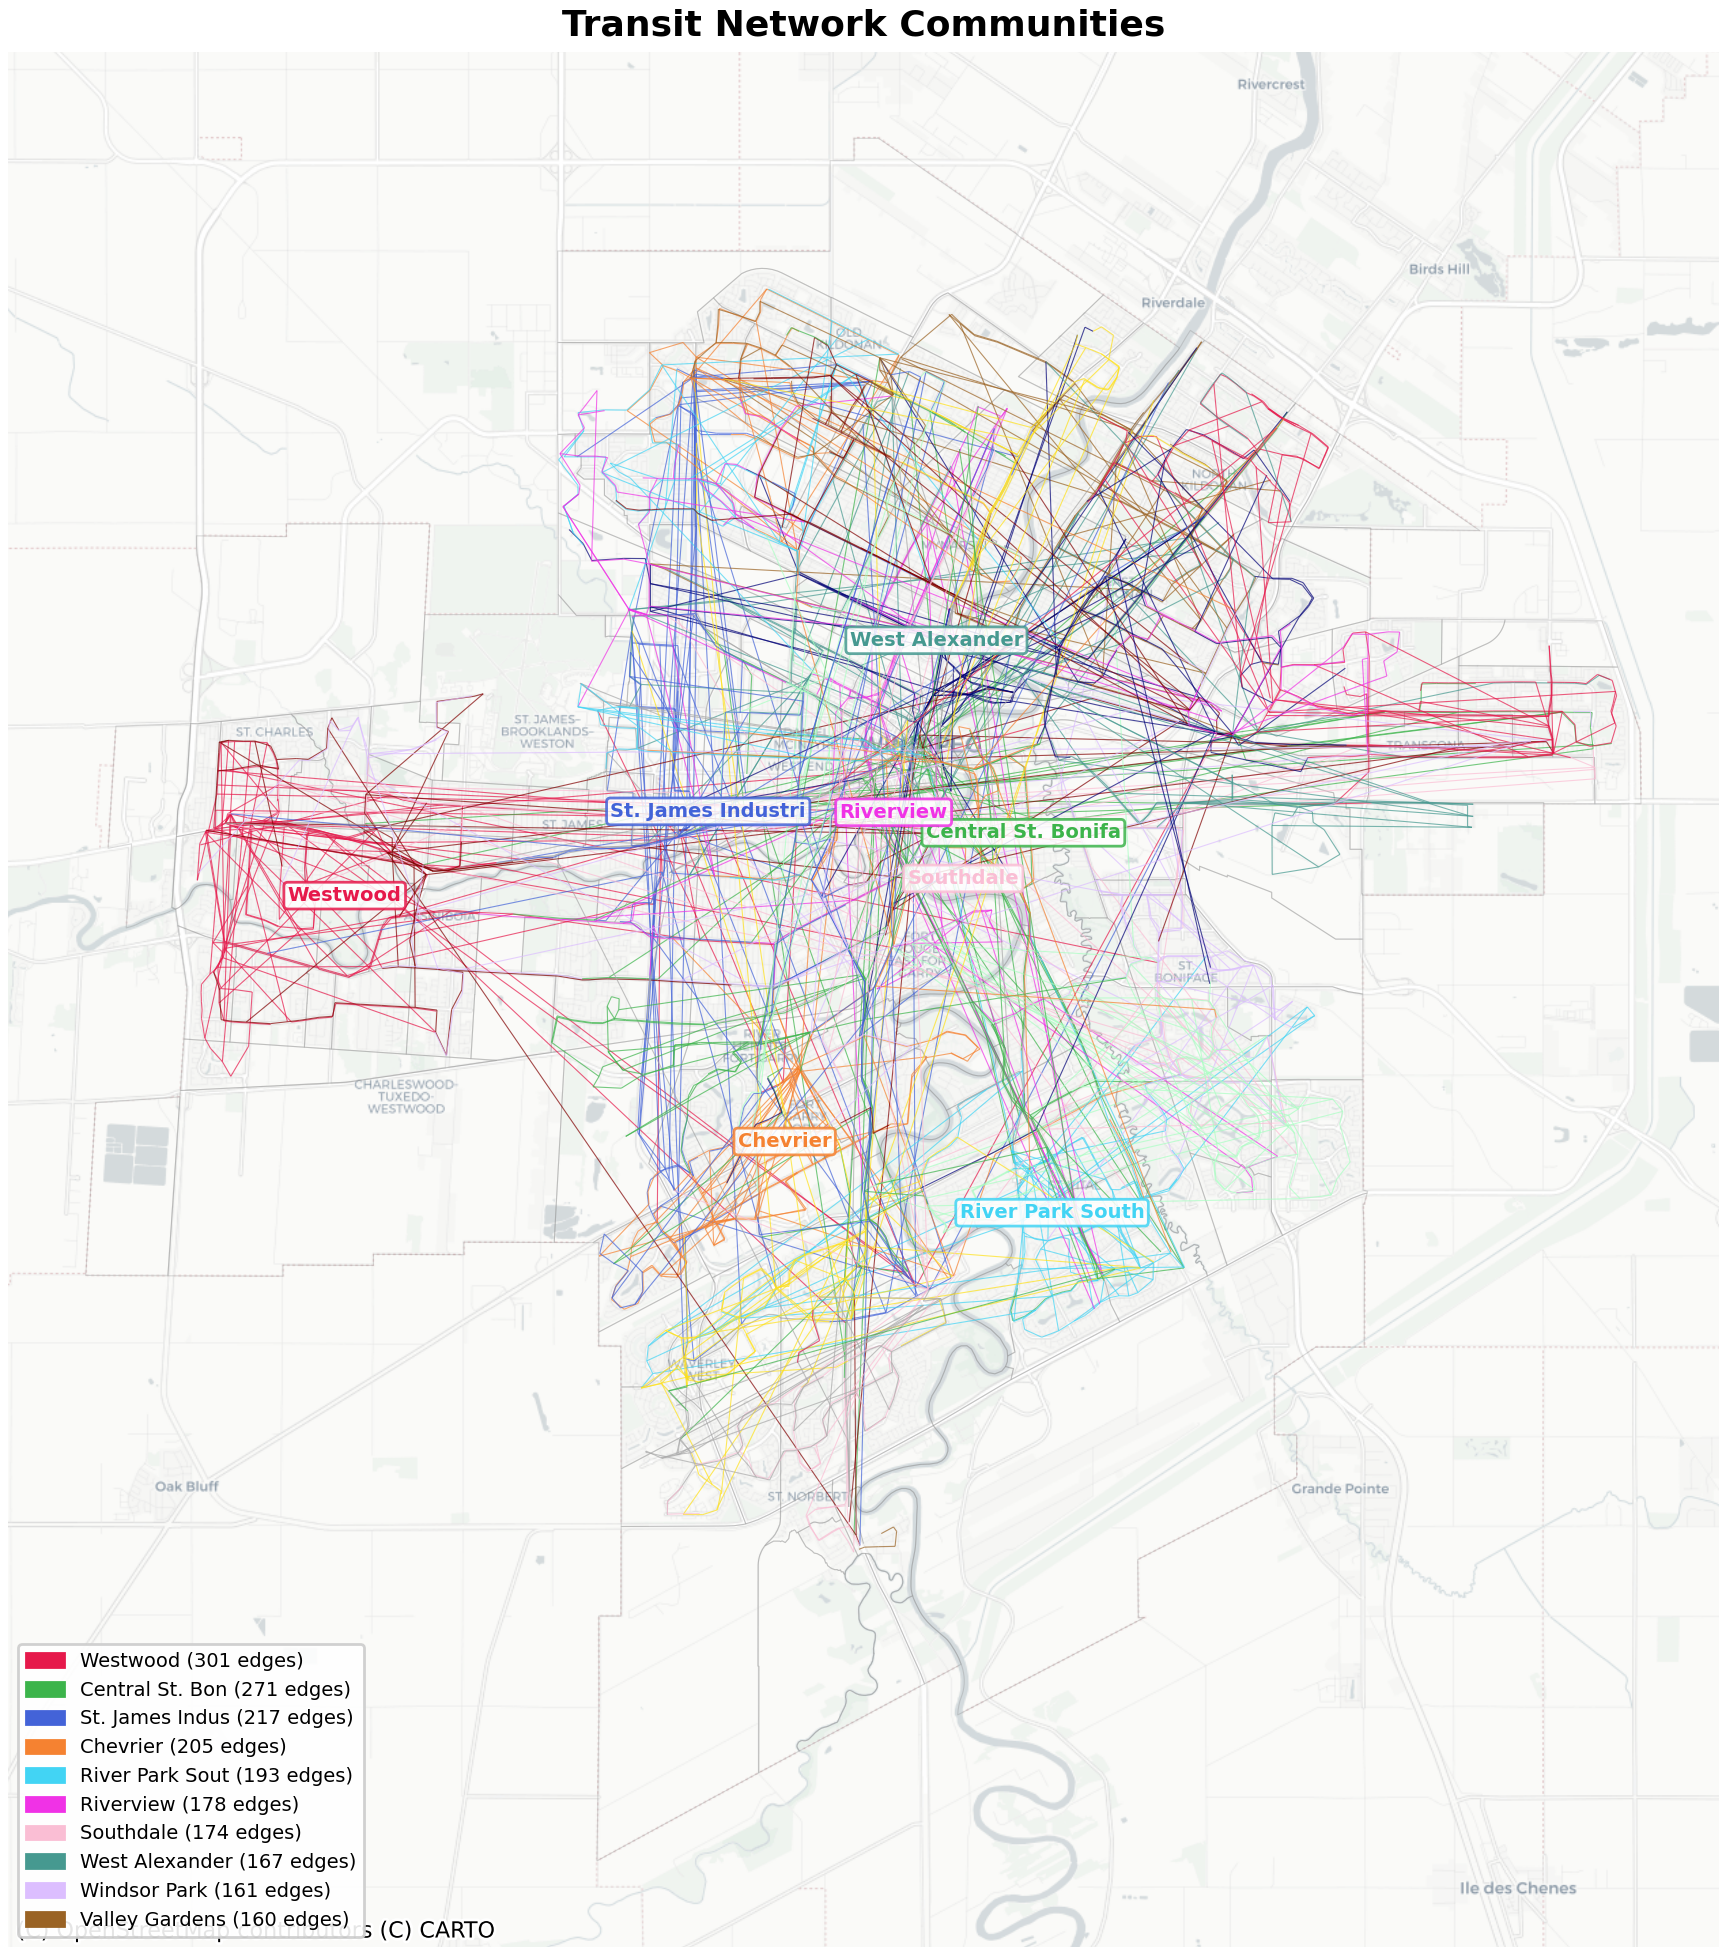
\includegraphics[width=\textwidth,height=7.5cm,keepaspectratio]{network_communities_pr2.png}
        \caption{Transit network communities (edge-coloured).}
        \label{fig:network_communities}
    \end{subfigure}
    \caption{Community detection: (a) Louvain clusters overlaid on neighbourhood boundaries (Cathy); (b) stop-to-stop edges coloured by community (Stephenie).}
\end{figure}

% ----------------------------------------
\subsection{Coverage \& Equity (Sudipta)}

Sudipta has attended all group meetings and contributed to coverage analysis discussions throughout the project.  His planned deliverables (a coverage change choropleth comparing pre-PTN and current stop density, and an underserved neighbourhood ranking with equity cross-tabulation) were not completed in time for this report due to complications with the data pipeline rebuild and Git LFS storage issues that consumed significant debugging time in the final week.  The full coverage analysis will be completed for the final report.

% ----------------------------------------
\subsection{Visualization Summary (Stephenie)}

Stephenie assembled summary visualizations that package analytical results for non-technical interpretation. Figure~\ref{fig:summary_panel} aggregates headway, speed, and route counts by PTN tier alongside the before/after route comparison. Figure~\ref{fig:network_communities} colours stop-to-stop edges by Louvain community to reveal the transit system's spatial clustering structure.

\begin{figure}[H]
    \centering
    \begin{subfigure}[t]{0.58\textwidth}
        \centering
        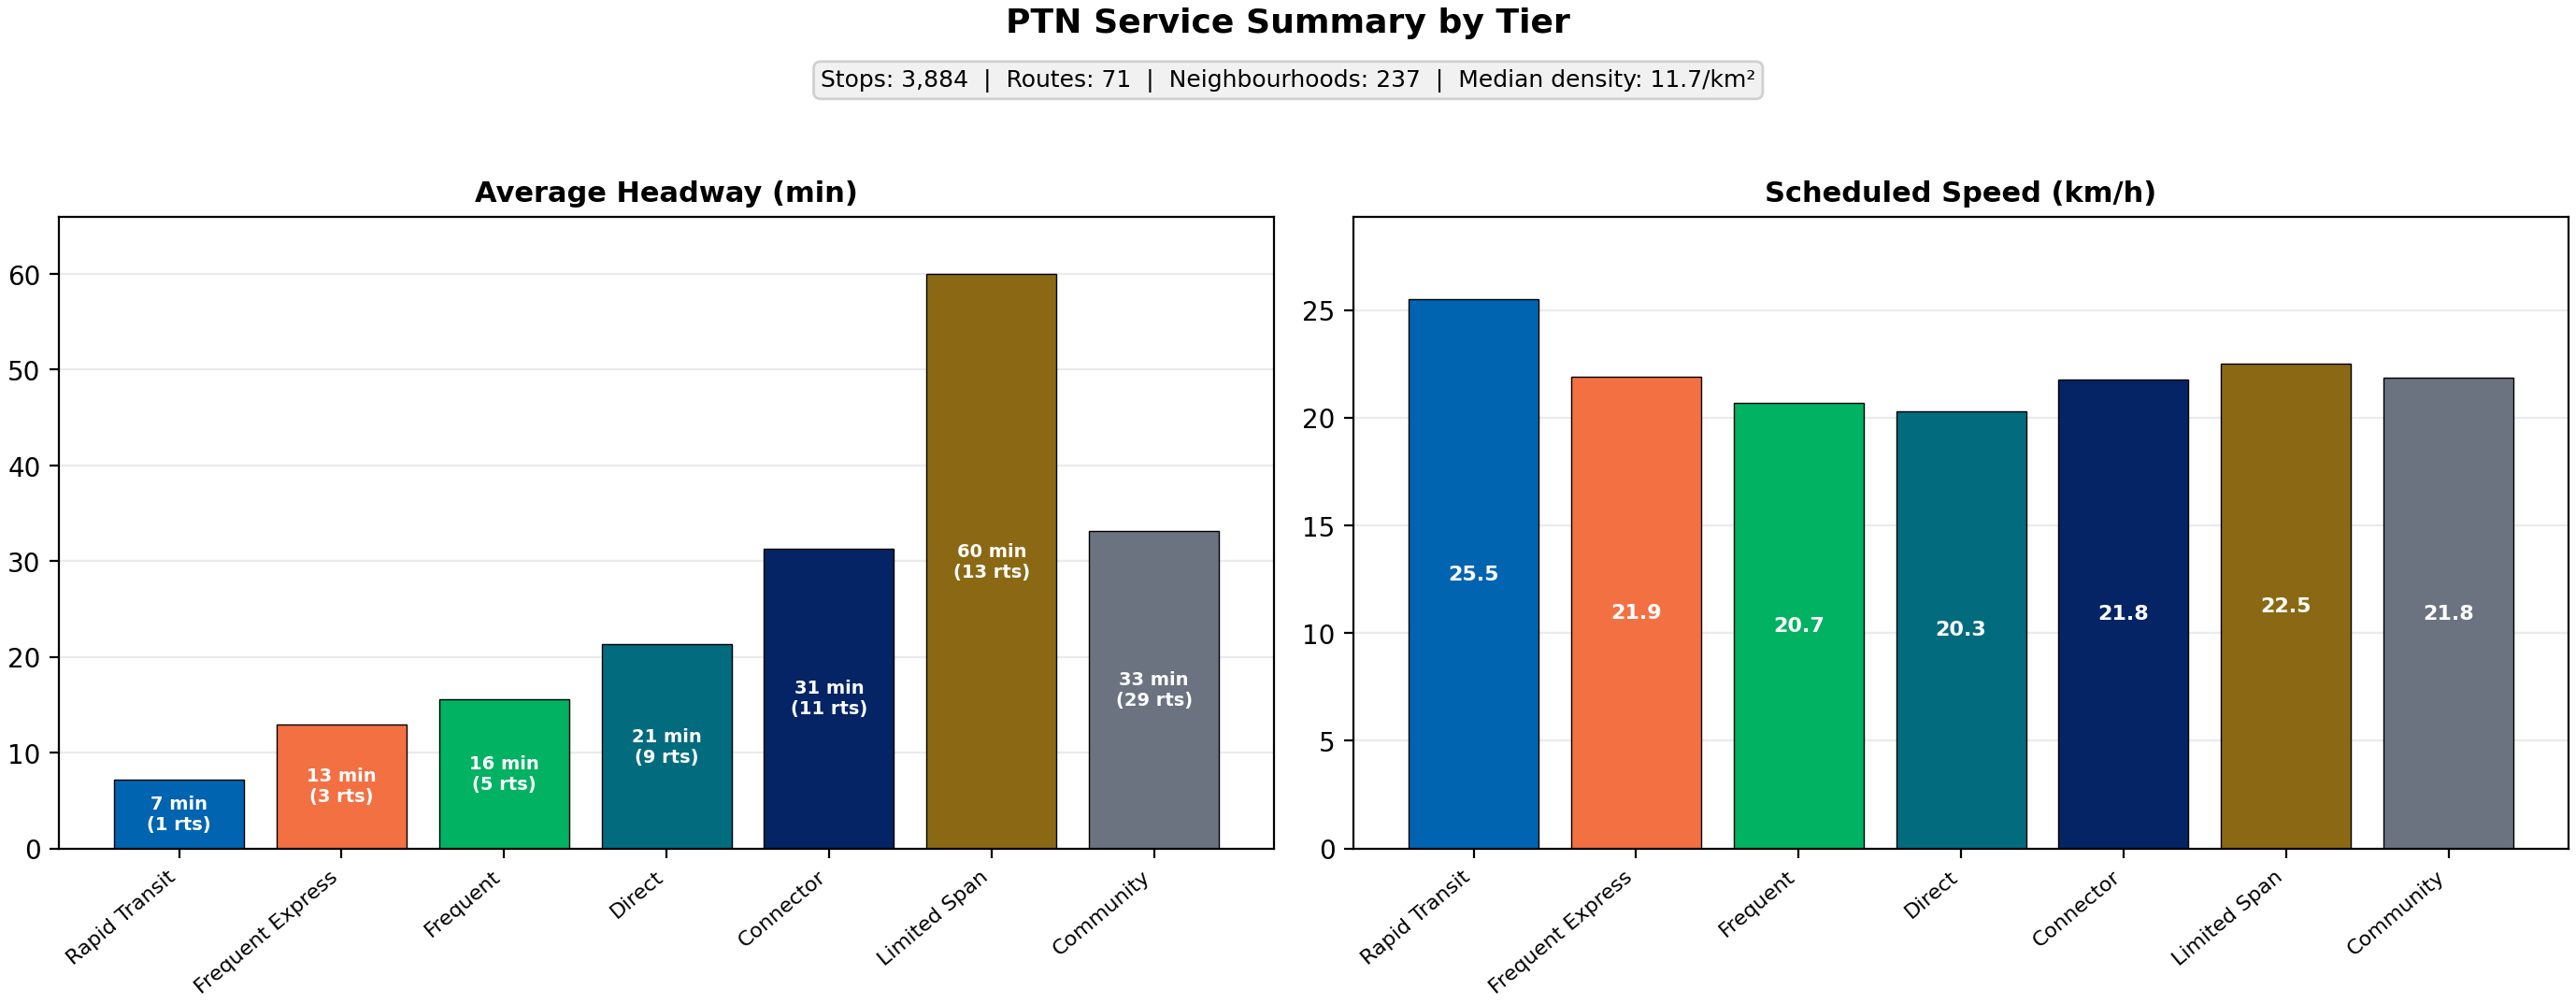
\includegraphics[width=\linewidth]{pr2_summary_panel.png}
        \caption{KPI summary by PTN tier with route counts.}
    \end{subfigure}\hfill
    \begin{subfigure}[t]{0.38\textwidth}
        \centering
        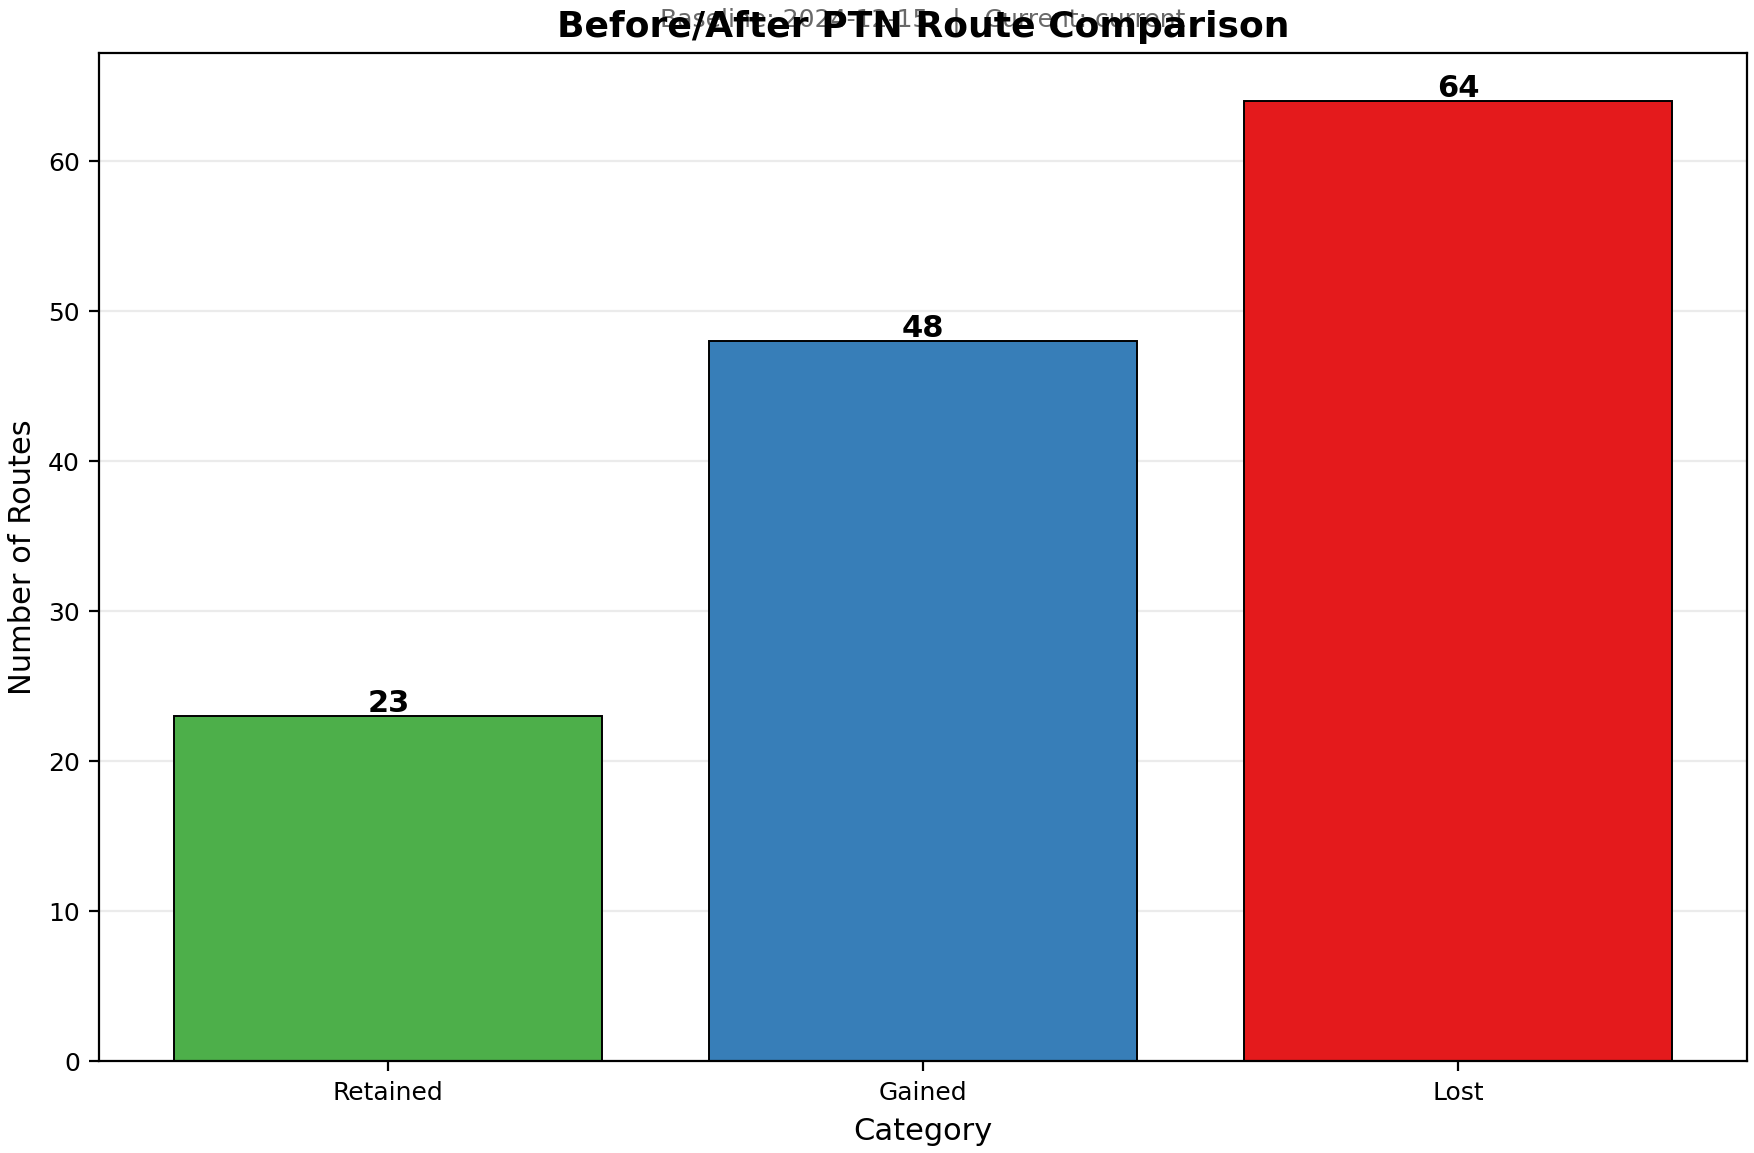
\includegraphics[width=\linewidth]{before_after_routes.png}
        \caption{Routes retained, gained, and lost.}
    \end{subfigure}
    \caption{Service summary and route retention analysis.}
    \label{fig:summary_panel}
\end{figure}

% ----------------------------------------
\subsection{Challenges and Mitigation}

\begin{table}[H]
\centering\scriptsize
\renewcommand{\arraystretch}{1.05}
\begin{tabularx}{\textwidth}{@{}l X@{}}
\toprule
\textbf{Challenge} & \textbf{Resolution} \\
\midrule
Route identity across PTN redesign & Jaccard stop-set matching; 55 exact-name + overlap-matched routes \\
Git LFS quota exceeded & Large binary files (DuckDB, parquet) exceeded GitHub LFS bandwidth; switched to \texttt{.gitignore} with \texttt{make data} rebuild \\
Pipeline rebuild cost & Full rebuild takes $\sim$50 minutes with API rate limits; added \texttt{pooch} caching and incremental table checks \\
Census DA geometry joins & CHASS CSV joined to Open Data boundaries via spatial intersection \\
Schedule-based analysis only & GTFS schedules used; no real-time vehicle tracking available \\
Employment data proxy & Business register establishment counts used in place of commute flows \\
Census 2021 income timing & Income reference year is 2020 (COVID year); interpret with caution \\
PTN still evolving & Results represent a transitional snapshot; network changes are ongoing \\
\bottomrule
\end{tabularx}
\caption{Challenges encountered, limitations, and resolutions applied.}
\label{tab:challenges}
\end{table}

\vspace{-0.3em}

% ============================================================
\section{Updated Plan and Timeline}

Core pipeline and analysis modules are complete.  Remaining work focuses on the interactive dashboard, presentation preparation, Sudipta's coverage figures, and final report assembly.

\begin{table}[H]
\centering\scriptsize
\renewcommand{\arraystretch}{1.05}
\begin{tabularx}{\textwidth}{@{}l l X X X X@{}}
\toprule
\textbf{Period} & \textbf{Milestone} & \textbf{Ahmed} & \textbf{Cathy} & \textbf{Stephenie} & \textbf{Sudipta} \\
\midrule
Jan 20 -- Feb 7 & PR1 \checkmark & GTFS pipeline, frequency module & Network module, graph stats & Visualizations, interactive maps & Coverage analysis, density stats \\
\addlinespace
Feb 10 -- Mar 13 & PR2 \checkmark & Pre/post comparison, clustering, classification, capacity & Pre/post network metrics, transfer heatmap & Summary panel, coverage cluster map & Coverage change choropleth \\
\addlinespace
Mar 14 -- 30 & Polish & Finalize figures; dashboard & Presentation slides & Dashboard styling; presentation visuals & Complete coverage figures; slides \\
\addlinespace
Mar 31 -- Apr 5 & Final & Methodology writeup; report assembly & Network section writeup & Report formatting \& final edits & Coverage section writeup \\
\addlinespace
\textbf{April 6} & \textbf{Final due} & Submit & Submit & Submit & Submit \\
\addlinespace
Apr 7 -- 9 & Presentation & Technical accuracy & Network slides & Design \& visuals & Coverage slides \\
\bottomrule
\end{tabularx}
\caption{Updated project timeline with per-member task allocation.}
\label{tab:timeline}
\end{table}

\vspace{-0.3em}

% ============================================================
\section{Acknowledgement}

No assistance was received from the TA in preparing this report.  We thank the City of Winnipeg Open Data Portal and Winnipeg Transit for providing publicly available datasets. We also acknowledge Statistics Canada (Census 2021), the CHASS Census Analyser (University of Toronto), and Innovation, Science and Economic Development Canada (Canadian Business Patterns).

\vspace{-0.3em}

% ============================================================
\section{Consent Declaration}

We, the undersigned, have reviewed this document and consent to submit it as Progress Report 2 for our group project.

\begin{table}[H]
\centering
\begin{tabular}{l l l}
\toprule
\textbf{Member} & \textbf{Initials for Signature} & \textbf{Date} \\
\midrule
Ahmed Hasan & ASH & March 12, 2026 \\
Cathy Li & CL & March 12, 2026 \\
Stephenie Michael & SCM & March 12, 2026 \\
Sudipta Sarker & SS & March 12, 2026 \\
\bottomrule
\end{tabular}
\end{table}

\vspace{-0.3em}

% ============================================================
\appendix
\section{References \& Datasets}

\scriptsize
\begin{itemize}[leftmargin=*,itemsep=0pt]
    \item Winnipeg Transit. ``GTFS Feed.'' \url{https://winnipegtransit.com/en/schedules-maps-tools/open-data/}
    \item City of Winnipeg. ``Open Data Portal.'' \url{https://data.winnipeg.ca/}
    \item Statistics Canada. ``Census Profile, 2021 Census of Population.'' Catalogue no.\ 98-316-X2016001. Dissemination area level. Accessed via CHASS Census Analyser, University of Toronto, March 2026.
    \item CHASS Data Centre, University of Toronto. ``Census Analyser.'' \url{https://dc.chass.utoronto.ca/census/}
    \item Innovation, Science and Economic Development Canada. ``Canadian Business Patterns (CBP), December 2022.'' Dissemination area level establishment counts.
    \item J.\ Allen \& S.\ Farber. ``Planning transport for social inclusion.'' \textit{Transportation Research Part D}, 2020.
    \item G.\ Boeing. ``Street Network Models and Indicators for Every Urban Area in the World.'' \textit{Geographical Analysis}, 2021.
    \item S.\ Ho. \textit{Identifying clusters of transit unreliability through an equity lens: Winnipeg, Manitoba}. Western University, 2024.
    \item M.\ Iacono, K.\ Krizek \& A.\ El-Geneidy. ``Measuring Non-Motorized Accessibility.'' \textit{J.\ Transport Geography}, vol.\ 18, pp.\ 133--140, 2010.
    \item S.\ Chicken. ``Why Winnipeg doesn't know who's riding the bus.'' \textit{The Narwhal}, 2024.
    \item T.\ Bao et al. ``PubtraVis: Public transit visualization.'' \textit{ISPRS Int.\ J.\ Geo-Inf.}, vol.\ 9, no.\ 4, 2020.
    \item TRB. \textit{Transit Capacity and Quality of Service Manual} (TCQSM), 3rd ed., 2013. 400\,m pedestrian catchment standard.
    \item WalkScore. ``Transit Score Methodology.'' \url{https://www.walkscore.com/methodology.shtml}, 2011.
    \item C.\ Fink et al. ``r5py: Rapid Realistic Routing with R5 in Python.'' \url{https://r5py.readthedocs.io/}, 2022.
    \item Y.\ Yuan et al. ``city2graph: From urban spatial data to graph representations.'' \url{https://github.com/c2g-dev/city2graph}, 2024.
    \item Hagberg, A., Schult, D.\ \& Swart, P. ``NetworkX.'' \url{https://networkx.org/}
    \item Jordahl, K.\ et al. ``GeoPandas.'' \url{https://geopandas.org/}
    \item DuckDB Foundation. ``DuckDB: In-process SQL OLAP database.'' \url{https://duckdb.org}
    \item MRCagney. ``gtfs-kit: A Python toolkit for GTFS feeds.'' \url{https://github.com/mrcagney/gtfs_kit}
    \item Pedregosa, F.\ et al. ``Scikit-learn: Machine Learning in Python.'' \textit{JMLR}, vol.\ 12, 2011.
\end{itemize}

\end{document}
